\documentclass[11pt,a4paper,openany]{report}
\usepackage[T1]{fontenc}
\usepackage[utf8]{inputenc}
\usepackage{lmodern}
\usepackage{microtype}
\usepackage{amsmath,amssymb,amsthm,mathtools,bm}
\usepackage{booktabs,array,longtable,tabularx}
\usepackage{xcolor}
\usepackage[margin=23mm,headheight=23pt]{geometry}
\usepackage{enumitem}
\usepackage{fancyhdr}
\usepackage{fancyvrb}
\usepackage{graphicx}
\usepackage{url}
\usepackage{xurl}
\usepackage{hyperref}

\definecolor{finblue}{HTML}{1F5A99}
\definecolor{fingreen}{HTML}{19733A}
\definecolor{finorange}{HTML}{D55E00}
\definecolor{finred}{HTML}{A61B1B}
\definecolor{finviolet}{HTML}{6A3D9A}
\definecolor{fingray}{HTML}{4D4D4D}

\hypersetup{
  unicode=true,
  colorlinks=true,
  linkcolor=finblue,
  citecolor=fingreen,
  urlcolor=finblue,
  pdftitle={FIN Laboratory Transfer Package: P240 Optimal Tomography, P241 Validator, P242 One-Shot Pipeline},
  pdfauthor={Krzysztof Żuchowski},
  pdfsubject={Scientific transfer package and executable specification for a blind twelve-state FIN laboratory experiment},
  pdfkeywords={FIN, heat-kernel tomography, continuous-time quantum walk, Markov semigroup, photonics, double slit, blind custody, preregistration, spectral fingerprint}
}

\pagestyle{fancy}
\fancyhf{}
\fancyhead[L]{\small FIN Laboratory Transfer Package}
\fancyhead[R]{\small Release 10.21}
\fancyfoot[C]{\thepage}
\setlength{\parindent}{0pt}
\setlength{\parskip}{0.55em}
\setlist{nosep,leftmargin=2em}
\setcounter{tocdepth}{2}
\setcounter{secnumdepth}{3}
\emergencystretch=3em

\newcommand{\one}{\bm 1}
\newcommand{\C}{\mathbb C}
\newcommand{\R}{\mathbb R}
\newcommand{\Z}{\mathbb Z}

\begin{document}
\hypersetup{pageanchor=false}
\begin{titlepage}
\centering
\vspace*{7mm}
{\Large\bfseries FIN Laboratory Transfer Package --- Release 10.21\par}
\vspace{10mm}
{\Huge\bfseries P240 Optimal Tomography\par}
\vspace{3mm}
{\Huge\bfseries + P241 Blind-Custody Validator\par}
\vspace{3mm}
{\Huge\bfseries + P242 One-Shot Pipeline\par}
\vspace{8mm}
{\Large A scientific transfer package and executable specification\\
for theoretical and experimental physicists\par}
\vspace{15mm}
{\Large Krzysztof \.Zuchowski\par}
\vspace{2mm}
{\normalsize Independent Researcher --- Fractal Information Theory Project\par}
\vspace{2mm}
{\normalsize ORCID: \href{https://orcid.org/0009-0002-0909-3613}{0009-0002-0909-3613}\par}
\vspace{8mm}
{\large 27 July 2026\par}
{\normalsize Publication --- Preprint and executable specification; version 1.0.0\par}
\vfill
\begin{minipage}{0.91\textwidth}
\small
\textbf{Transfer target.} One finite, calibrated, twelve-state laboratory
test of the strict FIN generator, with an independently signed event bundle,
a sealed \(2\tau\) holdout and exactly one registered analysis.

\medskip
\textbf{Central mathematical object.}
\[
W=K_s,\qquad s=1.660307278766099,\qquad
A=sI-W\geq0,\qquad U_t=e^{-itA},\quad P_t=e^{-tA}.
\]

\textbf{Critical boundary.} This package supplies a design, validator and
analysis pipeline. It supplies no external events, physical clock, apparatus,
strict selector, legacy--strict role transfer, \(L_{\rm total}\), Standard
Model/gravity derivation or Theory-of-Everything closure.

\medskip
\textbf{Repository.}
\url{https://github.com/hyconiek/Fractal-Nadsoliton-Theory}

\textbf{Related project DOI supplied by the author.}
\url{https://doi.org/10.5281/zenodo.21435332}

\textbf{License.} Creative Commons Attribution 4.0 International (CC BY 4.0).
\end{minipage}
\vfill
\end{titlepage}
\hypersetup{pageanchor=true}

\pagenumbering{roman}
\chapter*{Transfer statement}
\addcontentsline{toc}{chapter}{Transfer statement}
This document is intended to be handed, together with the hashed executable
files, to a laboratory team.  It summarizes the finite spectral theory,
the wave--diffusion duality, the missing operational object, the three
candidate apparatus classes, the registered acquisition design, the
independent custody contract and the one-shot analysis rule.

Programs 240--242 in this document are laboratory programme numbers from the
Release-10.20 roadmap.  They are not the older internal FAR packets that
happen to contain the same integers.

\tableofcontents
\clearpage
\pagenumbering{arabic}

\section{Confidence convention}

Analytic proof, machine checking, synthetic planning, feasibility hypotheses, open obligations and scoped refutations are kept separate throughout this transfer package.

\chapter{Abstract}

This document transfers the experimentally actionable part of the FIN research programme to an independent team of theoretical and experimental physicists. It begins from the finite strict twelve-node kernel, not from cosmological or Theory-of-Everything claims. With

\[
W=K_s,\qquad s=1.660307278766099,\qquad A=sI-W,
\]

the exact Dirichlet identity

\[
\langle f,Af\rangle
=
\frac12\sum_{x,y}W_{xy}|f_x-f_y|^2
\geq 0
\]

places the same self-adjoint generator under the coherent group

\[
U_t=e^{-itA}
\]

and the reversible heat/\allowbreak{}Markov semigroup

\[
P_t=e^{-tA}.
\]

This duality is mathematically proved on the frozen \(C_{12}\) target. It does not select which temporal law is physical. State space, preparation, clock, instrument, environment, apparatus, record and dimensional calibration remain operational inputs. The document therefore does not ask a laboratory to confirm a metaphysical interpretation. It asks whether an explicitly realized, calibrated and blinded twelve-state process follows the registered FIN transition law and whether it survives a one-time held-out semigroup test.

Program 240 is executed here. The fastest-mode inverse-log noise factor is \(e^x/x\), with the unique optimum

\[
x=\tau\lambda_{\max}=1.
\]

Cyclic symmetrization makes equal allocation to all twelve basis preparations minimax within the declared convex design class. A rectangular matrix-Bernstein theorem supplies a nonasymptotic spectral concentration bound. Synthetic planning gives a \(99\%\) and \(100\%\) pass rate for the frozen projective spectral gate at respectively \(25\,000\) and \(50\,000\) shots per preparation, while the fully distribution-free sufficient count for the same \(0.02\) projective bound is approximately \(22.6\) million per preparation. The large difference is reported, not hidden.

Program 241 is an executable blind-custody validator. It checks eleven measurement, data, calibration, control, chronology, hash and role-separation fields and requires a detached signature from a trusted registrar. It accepts either a twelve-state process record or an event-level double-slit record. It cannot generate the missing independent empirical record.

Program 242 is a fail-closed analysis pipeline. It runs exactly once for an admitted twelve-state process bundle, predicts

\[
P_{2\tau}^{\mathrm{pred}}=\widehat P_\tau^2,
\]

compares the prediction with the sealed \(\widehat P_{2\tau}\) holdout, evaluates the strict projective fingerprint and preregistered negative controls, and reports failure without model repair. No external bundle is supplied in this release; consequently Program 242 remains locked and no physical validation is claimed.

\par\medskip\hrule\medskip

\chapter{Executive decision for a laboratory team}

\section{What is ready}

\begin{itemize}
\item 
The finite strict target matrix and spectrum are frozen.

\item 
The dual unitary/\allowbreak{}heat mathematics is proved on that target.

\item 
The heat-kernel instrument-to-spectrum theorem is explicit.

\item 
P240 supplies the registered time, allocation, shot plan and concentration bounds.

\item 
P241 supplies a production validator, transfer template and signed-custody gate.

\item 
P242 supplies a one-run semigroup/\allowbreak{}fingerprint pipeline.

\item 
Eighteen regression tests pass.

\end{itemize}

\section{What is not ready}

\begin{itemize}
\item 
No external event bundle exists in this package.

\item 
No code can manufacture independent custody, an independent apparatus or a real physical preparation.

\item 
No laboratory is asserted to realize the twelve basis states, vertex POVM, or a homogeneous FIN semigroup.

\item 
No absolute physical time, energy, action or length unit follows from the dimensionless operator.

\item 
The strict selector obstruction QW-2191 remains open.

\item 
The legacy-to-strict completion bridge and legacy physical-role transfer remain open.

\item 
No \(L_{\rm total}\), Standard Model, general-relativistic or Theory-of-Everything closure is claimed.

\end{itemize}

\section{Platform recommendation}

\begin{center}
\begingroup\small
\setlength{\tabcolsep}{3.5pt}
\renewcommand{\arraystretch}{1.16}
\begin{longtable}{@{}p{0.311\textwidth}p{0.311\textwidth}p{0.238\textwidth}@{}}
\toprule
\textbf{Platform} & \textbf{Direct relevance to P227/\allowbreak{}P240--P242} & \textbf{Recommended role} \\
\midrule
\endhead
P-A: twelve-mode photonic coherent walk plus separately verified stochastic/\allowbreak{}open-system realization & high & primary FIN process experiment \\
P-B: qubit Mach--Zehnder/\allowbreak{}Ramsey single--plus--echo dephasing experiment & medium as an operational-method test; low as a twelve-node FIN test & auxiliary memory, dephasing and instrument validation \\
P-C: event-level single-photon double slit with four shutter configurations & high for event acquisition and custody; low for direct \(12\times12\) spectral reconstruction & procedural pilot and independent interference record \\
\bottomrule
\end{longtable}
\endgroup
\end{center}

The recommended scientific sequence is:

\begin{enumerate}
\item 
use P-C, if convenient, to prove that the collaboration can produce the required event-level, signed, blinded record;

\item 
execute P-A as the direct twelve-state process test;

\item 
use P-B only for auxiliary tests of dephasing, echo, memory and detector modelling;

\item 
do not treat a programmable emulator as evidence that nature selected FIN; it validates the implementation and falsification pipeline.

\end{enumerate}

\begin{figure}[htbp]
\centering
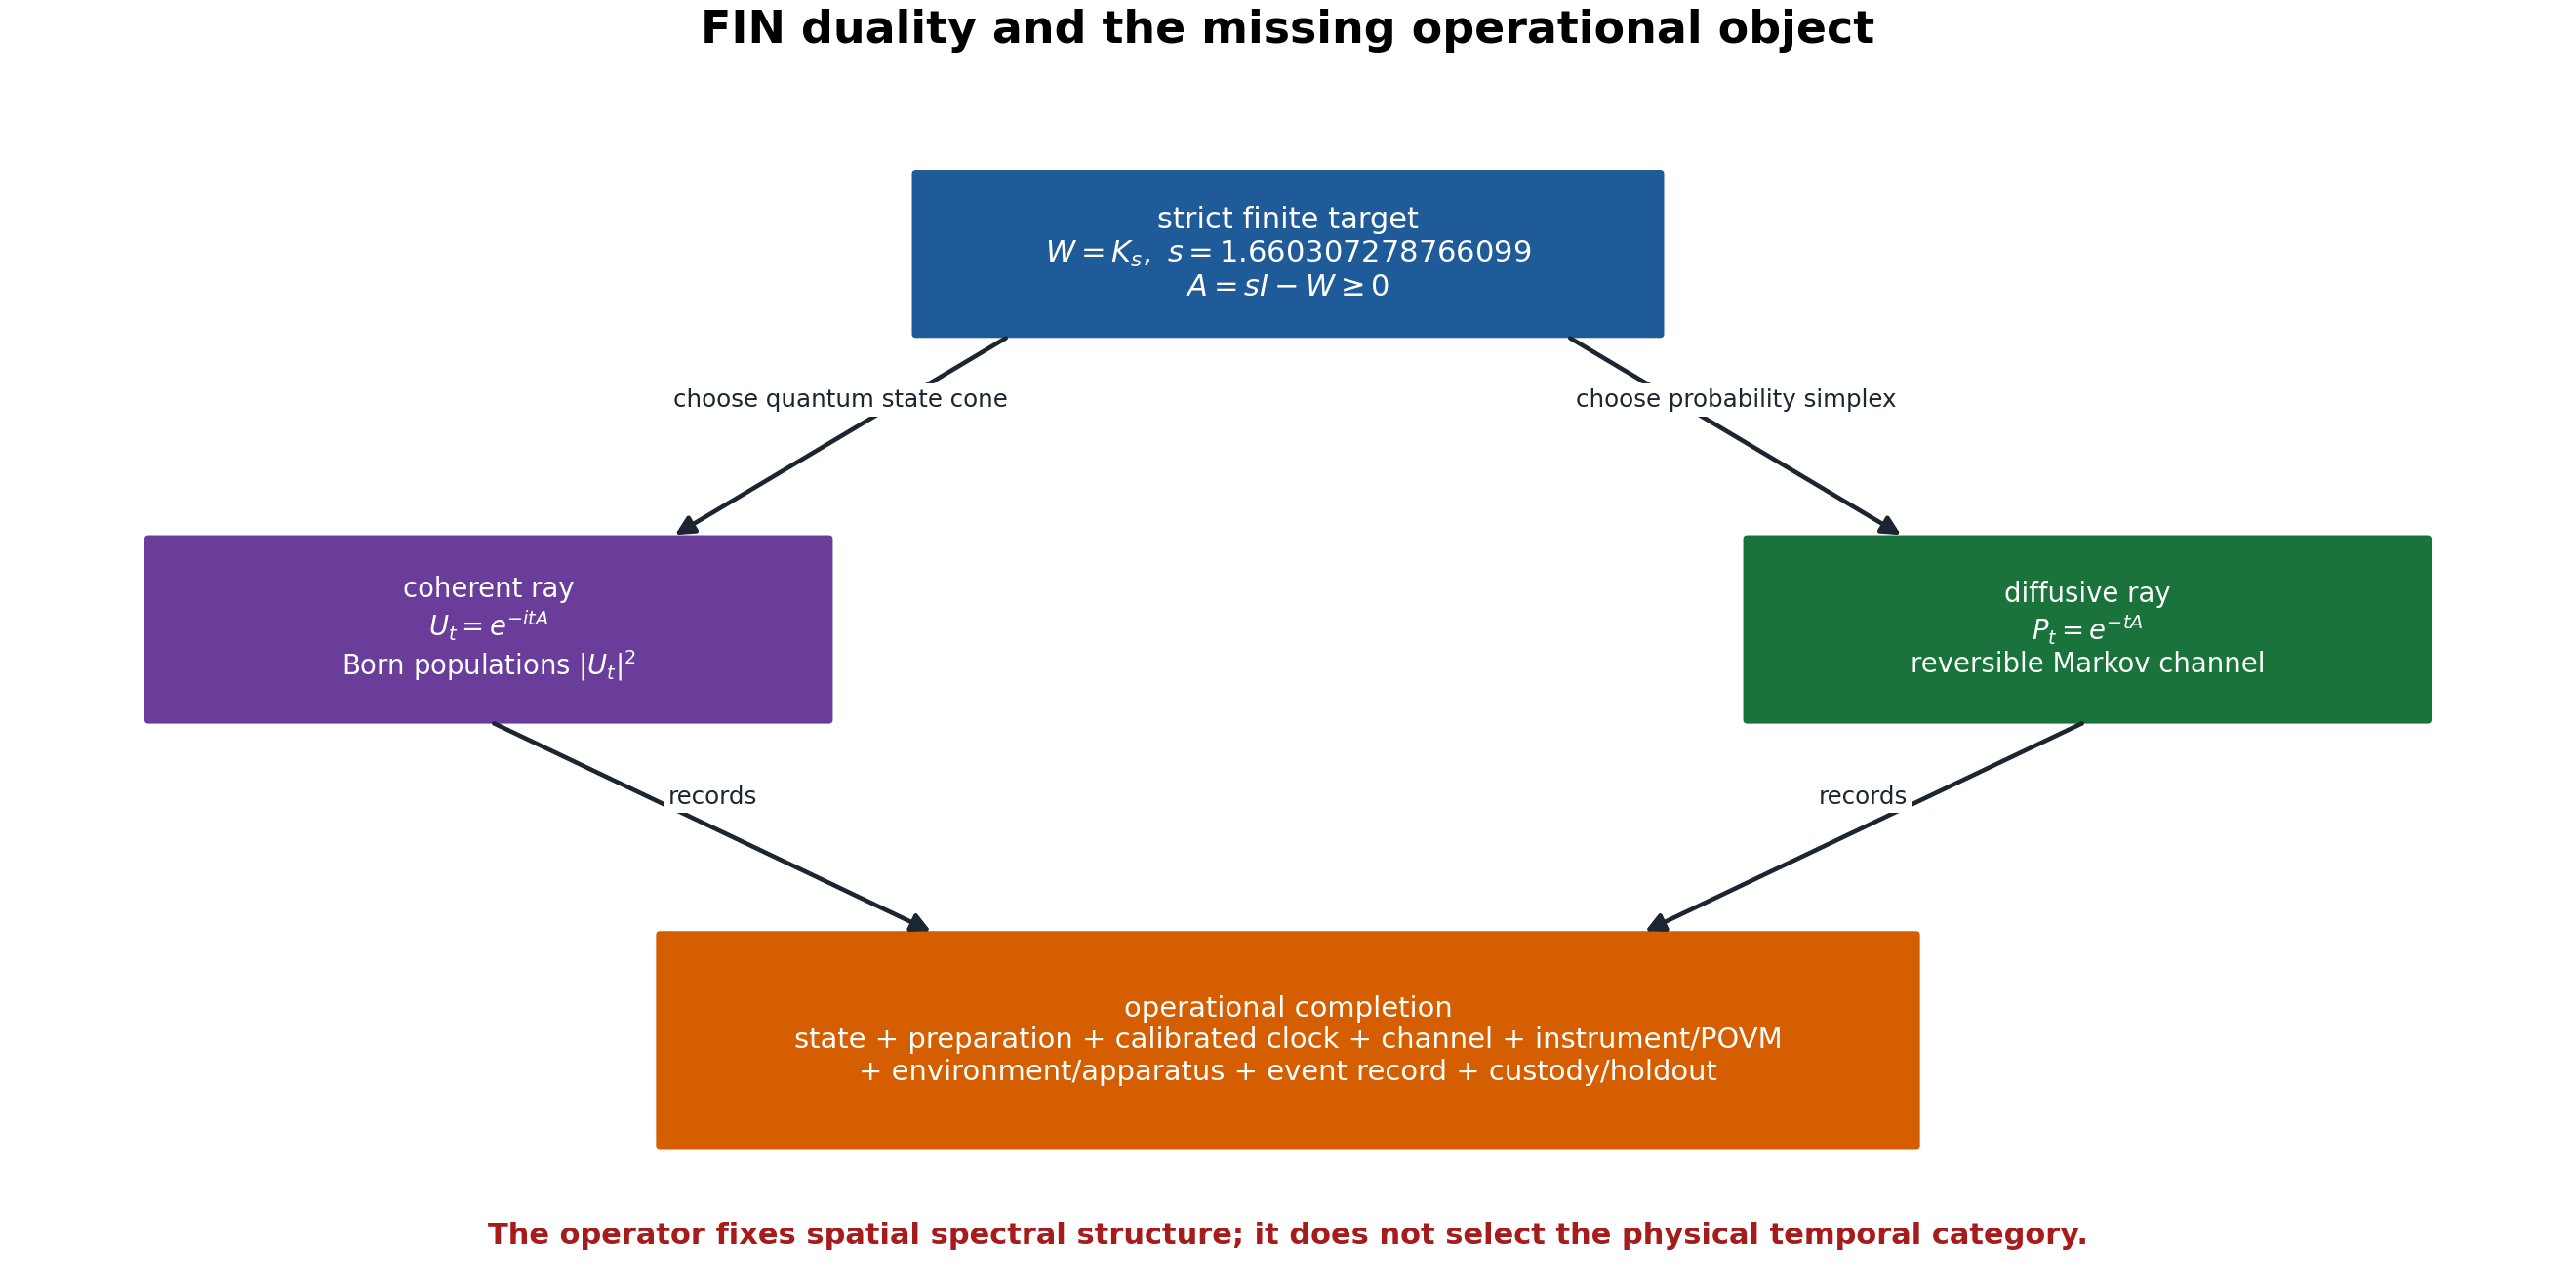
\includegraphics[width=0.96\textwidth]{FIN_Lab_P240_242_Transfer_Figures/duality_operational_map.png}
\caption{The same positive generator supports coherent and diffusive functional calculi, while empirical probabilities require an operational completion.}
\end{figure}

\par\medskip\hrule\medskip

\chapter{Claim convention}

\begin{center}
\begingroup\small
\setlength{\tabcolsep}{3.5pt}
\renewcommand{\arraystretch}{1.16}
\begin{longtable}{@{}p{0.420\textwidth}p{0.420\textwidth}@{}}
\toprule
\textbf{Label} & \textbf{Meaning} \\
\midrule
\endhead
\textbf{Proven} & analytic finite theorem in the declared scope \\
\textbf{Machine checked} & executable test or exact hash/\allowbreak{}schema check completed \\
\textbf{Synthetic planning evidence} & numerical experiment generated from a declared model; not physical evidence \\
\textbf{Feasibility hypothesis} & apparatus proposal requiring expert engineering review \\
\textbf{Open} & missing theorem, apparatus, calibration or external record \\
\textbf{Refuted in scope} & an explicit counterexample or no-go applies under stated assumptions \\
\bottomrule
\end{longtable}
\endgroup
\end{center}

No statement is promoted across these categories.

\par\medskip\hrule\medskip

\chapter{Scientific question}

The laboratory question is intentionally narrower than the overall FIN research programme:

\begin{quote}\itshape
Can an independently operated, calibrated twelve-state platform realize the frozen transition family associated with the strict FIN generator, and can its sealed \(2\tau\) record be predicted from its calibration-time \(\tau\) record without post-hoc repair?

\end{quote}

There are two associated but distinct questions:

\begin{enumerate}
\item 
does a coherent implementation realize the transition amplitudes of \(U_t=e^{-itA}\);

\item 
does a stochastic or open-system implementation realize the populations of \(P_t=e^{-tA}\)?

\end{enumerate}

The common generator makes these two calculations mathematically related. It does not make the two experimental procedures physically identical.

\par\medskip\hrule\medskip

\chapter{Frozen finite target}

\section{Strict working kernel}

Let \(V=\mathbb Z/12\mathbb Z\) and

\[
d(x,y)=\min\{|x-y|,12-|x-y|\}.
\]

The frozen strict working profile is

\[
K_{\rm strict}(d)
=
\frac{\cos(0.18575\,d+0.16250)}{1+d^{1.8}}.
\]

Define

\[
W_{xx}=0,\qquad
W_{xy}=K_{\rm strict}(d(x,y))
\quad(x\neq y).
\]

The six positive distance weights are

\begin{center}
\begingroup\small
\setlength{\tabcolsep}{3.5pt}
\renewcommand{\arraystretch}{1.16}
\begin{longtable}{@{}p{0.420\textwidth}p{0.420\textwidth}@{}}
\toprule
\textbf{\(d\)} & \textbf{\(K_{\rm strict}(d)\)} \\
\midrule
\endhead
1 & 0.46998567264502017 \\
2 & 0.19204355169010282 \\
3 & 0.09142861427792497 \\
4 & 0.04702916874565040 \\
5 & 0.02413122336363006 \\
6 & 0.011070817321442113 \\
\bottomrule
\end{longtable}
\endgroup
\end{center}

Every row has sum

\[
s=2\sum_{d=1}^{5}K_{\rm strict}(d)+K_{\rm strict}(6)
=1.6603072787660986,
\]

which agrees with the registered value \(1.660307278766099\) to \(4.44\times10^{-16}\).

\section{Positive Dirichlet generator}

Set

\[
A=sI-W.
\]

Because \(W\) is symmetric, nonnegative off diagonal and has constant row sum,

\[
\begin{aligned}
\langle f,Af\rangle
&=
s\sum_x|f_x|^2-\sum_{x,y}\overline f_xW_{xy}f_y\\
&=
\frac12\sum_{x,y}W_{xy}|f_x-f_y|^2
\geq0.
\end{aligned}
\]

Strict positivity of all off-diagonal weights makes

\[
\ker A=\operatorname{span}\{\mathbf 1\}.
\]

The nonnegative generator eigenvalues, organized by Fourier mode, are:

\begin{center}
\begingroup\small
\setlength{\tabcolsep}{3.5pt}
\renewcommand{\arraystretch}{1.16}
\begin{longtable}{@{}p{0.420\textwidth}p{0.420\textwidth}@{}}
\toprule
\textbf{Modes} & \textbf{\(\lambda(A)\)} \\
\midrule
\endhead
\(0\) & 0 \\
\(\pm1\) & 0.754121154207080 \\
\(\pm2\) & 1.577049514427610 \\
\(\pm3\) & 1.961406861976446 \\
\(\pm4\) & 2.199568849333210 \\
\(\pm5\) & 2.298606272079097 \\
\(6\) & 2.342182041146301 \\
\bottomrule
\end{longtable}
\endgroup
\end{center}

Thus

\[
\lambda_{\max}=2.342182041146298,
\qquad
\tau_*=\lambda_{\max}^{-1}=0.426952295949885
\]

in dimensionless FIN time.

\section{Kernel policy}

The laboratory target above is the later strict working kernel. It must not be silently identified with the canonical legacy intermediate kernel

\[
K_{\rm legacy}(d)
=
\alpha_{\rm geo}
\frac{\cos(\pi d/4+\pi/6)}{1+0.01d},
\qquad
\alpha_{\rm geo}=4\ln2.
\]

The current repository policy is:

\begin{itemize}
\item 
K\_strict\_gate is the primary strict finite target;

\item 
K\_legacy\_ont is an intermediate bridge kernel;

\item 
no raw identity, continuum completion theorem or physical-role transfer is available;

\item 
a fixed-support polynomial interpolation on \(C_{12}\) is not a universal completion law.

\end{itemize}

The laboratory must therefore label the implemented matrix explicitly and must not infer legacy electroweak, electromagnetic or gravity-role formulas from a strict-kernel fit.

\par\medskip\hrule\medskip

\chapter{One operator, multiple mathematical dynamics}

\section{Coherent group}

Self-adjointness gives

\[
U_t=e^{-itA},
\qquad
U_t^\dagger U_t=I,
\qquad
U_{t+u}=U_tU_u.
\]

If the initial amplitude is \(\psi_0\), then

\[
\psi(t)=U_t\psi_0.
\]

A vertex detector with effects \(E_x=|x\rangle\langle x|\) yields Born populations

\[
M_t(x|j)=|\langle x|U_t|j\rangle|^2.
\]

The matrices \(M_t\) are doubly stochastic at each fixed time, but generally

\[
M_{t+u}\neq M_tM_u.
\]

The missing cross terms are the finite interference witness.

\section{Diffusive semigroup}

Because \(Q=-A=W-sI\) has nonnegative off-diagonal entries and zero column and row sums,

\[
P_t=e^{tQ}=e^{-tA}
\]

is positive, symmetric, doubly stochastic and satisfies

\[
P_{t+u}=P_tP_u.
\]

Its stationary distribution is uniform. The spectral gap controls mixing:

\[
\|P_t-\Pi\|_{2\to2}=e^{-0.754121154207080\,t},
\qquad
\Pi=\frac1{12}\mathbf1\mathbf1^\mathsf T.
\]

\section{Short-time discriminator}

For a localized preparation \(j\) and \(i\neq j\),

\[
P_t(i|j)=W_{ij}t+O(t^2),
\]

whereas

\[
M_t(i|j)=W_{ij}^2t^2+O(t^4).
\]

Classical escape is linear and coherent escape is quadratic. A freely fitted clock can make one snapshot look similar, so the experiment must use a calibrated clock and multiple times.

\section{Wave, Green and variational shadows}

The same spectral measure also defines, when typed correctly:

\[
\cos(t\sqrt A),\qquad
\frac{\sin(t\sqrt A)}{\sqrt A},\qquad
(A+zI)^{-1},
\qquad
e^{-tA}.
\]

The quadratic functional

\[
S[\phi]
=
\frac12\phi^\mathsf TA\phi-J^\mathsf T\phi
\]

has stationary equation

\[
A\phi=J.
\]

This reconstructs a Green equation from the operator. It does not supply a physical action unit, a source \(J\), a Lorentzian continuum, gauge fields or a full field Lagrangian.

\section{The observer issue}

The two dynamics are not an observer-induced contradiction. They are two inequivalent temporal semantics of one spatial generator. The mathematical observer is an operationally specified apparatus:

\[
\mathcal P
=
(A,\mathcal S,\rho_0,\gamma,\{\Phi_\tau\},
\{\mathcal I_{a|x}\},F_{\rm app},\mathcal R).
\]

The entries denote generator, state/\allowbreak{}probability space, preparation, clock calibration, channel, instruments, apparatus frame and persistent record. Removing any entry creates a concrete nonidentifiability:

\begin{center}
\begingroup\small
\setlength{\tabcolsep}{3.5pt}
\renewcommand{\arraystretch}{1.16}
\begin{longtable}{@{}p{0.420\textwidth}p{0.420\textwidth}@{}}
\toprule
\textbf{Removed object} & \textbf{Failure} \\
\midrule
\endhead
state cone /\allowbreak{} probability rule & unitary and stochastic models remain possible \\
preparation & the uniform state hides both population dynamics \\
calibrated clock & rate and time can be inversely rescaled \\
instrument & intermediate observation and coherent propagation are conflated \\
environment & different memory/\allowbreak{}decoherence laws share terminal marginals \\
apparatus frame & odd/\allowbreak{}orientation data can be erased \\
record & no empirical likelihood or holdout exists \\
\bottomrule
\end{longtable}
\endgroup
\end{center}

This is why a fifth duty---an independent record and custody split---cannot be generated by the simulation code.

\par\medskip\hrule\medskip

\chapter{Dimensional and selector boundary}

The finite matrix \(A\) is dimensionless. Physical evolution would require, for example,

\[
U_{\tau_{\rm phys}}
=
\exp\!\left[-i\frac{E_0\tau_{\rm phys}}{\hbar}A\right],
\]

or

\[
P_{\tau_{\rm phys}}
=
\exp[-\kappa\tau_{\rm phys}A].
\]

Only \(E_0\tau_{\rm phys}/\hbar\) or \(\kappa\tau_{\rm phys}\) is visible to the dimensionless operator. The minimal conversion package remains

\[
\mathrm{CA}=(\ell_*,\tau_*,\hbar_*)
\]

or another independent rank-three basis of length, time and action/\allowbreak{}energy calibrations. It is imported through calibrated standards, not derived from a new dimensionless scalar.

Reflection exchanges Fourier modes \(+m\) and \(-m\). A radial operator cannot select an absolute orientation. A laboratory can supply a chiral preparation, directed apparatus or signed reference. That is an operational sector resource, not a strict-core discharge of QW-2191.

Shannon information computed from detector probabilities is dimensionless. Thermodynamic entropy, work and heat additionally require \(k_B\), a physical ensemble, temperature, Hamiltonian/\allowbreak{}bath and work/\allowbreak{}heat instruments. The experiment below does not silently make that conversion.

\par\medskip\hrule\medskip

\chapter{The exact empirical target}

\section{Primary heat-process prediction}

The calibration record estimates

\[
\widehat P_\tau.
\]

Without using the sealed \(2\tau\) data, Program 242 freezes

\[
\widehat P_{2\tau}^{\rm pred}
=
\widehat P_\tau\widehat P_\tau.
\]

The held-out statistic is

\[
T_{\rm CK}
=
\max_j
\operatorname{TV}
\left(
\widehat P_{2\tau}(\cdot|j),
\widehat P_\tau^2(\cdot|j)
\right).
\]

This is a Chapman--Kolmogorov/\allowbreak{}time-homogeneity test. A failure rejects the registered semigroup realization at the declared level. A non-rejection does not prove that nature selected FIN.

\section{Secondary projective spectral fingerprint}

For exact heat data,

\[
A=-\frac1\tau\log P_\tau.
\]

If the physical clock scale is unknown but stable, transition eigenvalues

\[
\mu_k=e^{-\tau\lambda_k}
\]

still determine

\[
\frac{\lambda_k}{\lambda_{\max}}
=
\frac{\log\mu_k}{\log\mu_{\min}}.
\]

The frozen secondary distance is the maximum absolute deviation between the reconstructed positive eigenvalue ratios and the strict target. The raw gate is \(0.02\).

\section{Coherent duality diagnostics}

If a coherent arm is available, it should additionally measure:

\begin{enumerate}
\item 
localized escape at \(\tau/4,\tau/2,\tau\);

\item 
\(M_{2\tau}-M_\tau^2\) with and without an intermediate vertex measurement;

\item 
phase-sensitive interference, not populations alone;

\item 
apparatus-reflection and preparation-label controls.

\end{enumerate}

The heat arm must not be inferred merely from loss of coherent visibility.

\par\medskip\hrule\medskip

\chapter{SECTION C --- PROPOSED EXPERIMENT AND APPARATUS}

\chapter{Five mandatory measurement duties}

The five duties from Program 227 and the Program-228 intake gate are:

\begin{center}
\begingroup\small
\setlength{\tabcolsep}{3.5pt}
\renewcommand{\arraystretch}{1.16}
\begin{longtable}{@{}p{0.055\textwidth}p{0.342\textwidth}p{0.284\textwidth}p{0.178\textwidth}@{}}
\toprule
\textbf{No.} & \textbf{Duty} & \textbf{Current mathematical status} & \textbf{Can code supply it?} \\
\midrule
\endhead
1 & vertex-basis or informationally complete preparations & explicit instrument model and design theorem & code specifies; laboratory must realize \\
2 & calibrated duration \(\tau\) & exact dimensionless optimum and calibration obligation & code specifies; external clock supplies units \\
3 & vertex-resolving measurement /\allowbreak{} vertex POVM & exact instrument-to-spectrum theorem & code specifies; apparatus must realize and calibrate \\
4 & finite transition counts & nonasymptotic and simulated shot analysis & code analyzes; detector supplies events \\
5 & independent record, holdout and provider--registrar--analyst separation & schema, validator and one-run gate only & \textbf{no}; this field is empirically empty until humans supply it \\
\bottomrule
\end{longtable}
\endgroup
\end{center}

Duties 1--4 have a theorem or a declared operational model. Duty 5 is not a software artifact and must not be filled with synthetic data, a screenshot, a rendered plot or a record produced by the same analysis team.

\begin{figure}[htbp]
\centering
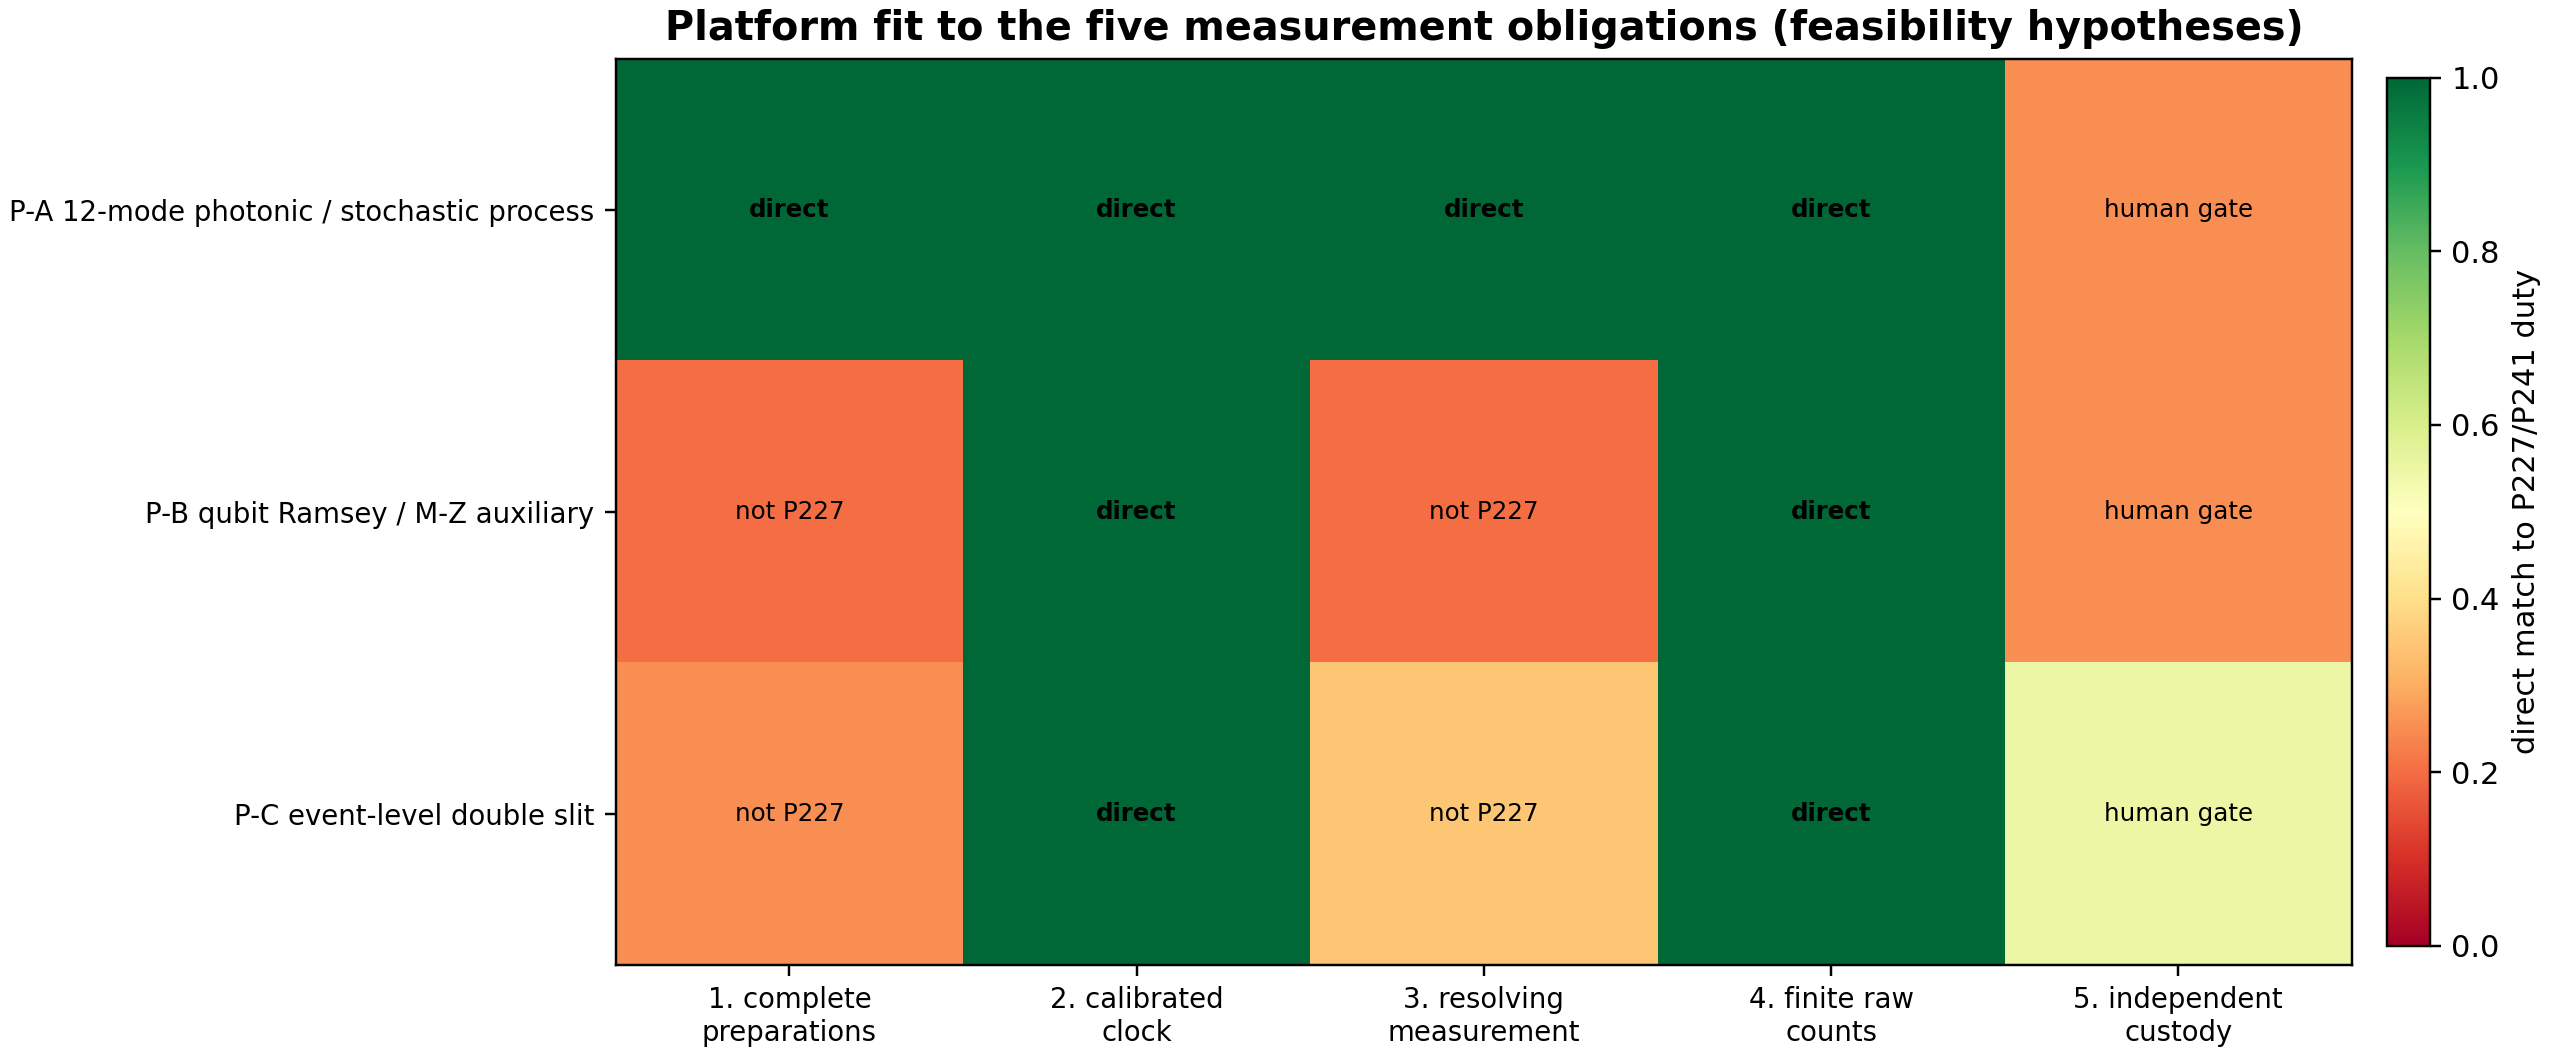
\includegraphics[width=0.96\textwidth]{FIN_Lab_P240_242_Transfer_Figures/platform_obligation_matrix.png}
\caption{Fit of the three feasibility hypotheses to the five measurement duties. Independent custody remains a human and institutional gate.}
\end{figure}

\chapter{Platform P-A --- twelve-mode photonic continuous-time walk}

\section{Feasibility status}

\textbf{Feasibility hypothesis, not a FIN theorem.} Integrated waveguide arrays and programmable multiport interferometers can realize large coherent mode networks. Controlled noisy quantum walks and event-resolved photonic measurements also exist. These precedents make a twelve-mode implementation plausible. They do not prove that a given chip realizes the FIN matrix.

\section{Apparatus}

\begin{itemize}
\item 
heralded single-photon source based on SPDC, or a strongly attenuated laser with documented photon statistics and a separate classical-intensity calibration;

\item 
source trigger and time-tagger reference;

\item 
twelve independently selectable input modes;

\item 
either femtosecond-laser-written waveguides or a reconfigurable Mach--Zehnder mesh implementing the coherent target;

\item 
calibrated phase shifters and coupling characterization;

\item 
an engineered dissipative/\allowbreak{}stochastic realization with transition rates \(W_{xy}\), for example explicit Lindblad jumps

\[
L_{xy}=\sqrt{W_{xy}}\,|x\rangle\langle y|,
\]

or a separately programmed stochastic router;

\item 
twelve SPAD or SNSPD output channels;

\item 
TCSPC/\allowbreak{}time-tagger electronics;

\item 
power, temperature, vibration and phase-stability monitors;

\item 
independent calibration paths for detector efficiency, dark counts, crosstalk and timing jitter;

\item 
shuttered/\allowbreak{}dark and nearest-neighbour controls.

\end{itemize}

\section{Critical correction to the proposed setup}

Ordinary propagation loss, pure dephasing or uncontrolled disorder does not by itself prove

\[
\dot p=-Ap.
\]

A passive lossy optical amplitude generally follows a non-Hermitian amplitude equation, and detected intensities are squared amplitudes. They are not automatically the columns of \(e^{-\tau A}\). The heat arm must therefore be derived from explicit jump/\allowbreak{}routing dynamics or independently reconstructed by process tomography.

\section{Mapping to the five duties}

\begin{center}
\begingroup\small
\setlength{\tabcolsep}{3.5pt}
\renewcommand{\arraystretch}{1.16}
\begin{longtable}{@{}p{0.420\textwidth}p{0.420\textwidth}@{}}
\toprule
\textbf{Duty} & \textbf{P-A implementation} \\
\midrule
\endhead
1 & inject each of the twelve input ports in randomized order \\
2 & calibrate propagation/\allowbreak{}coupling time or programmed transition duration against an external clock \\
3 & twelve resolved output channels; characterize confusion/\allowbreak{}crosstalk matrix \\
4 & retain every timestamped detector event and run identifier \\
5 & provider exports signed raw bundle to an independent registrar; analyst receives sealed split only through protocol \\
\bottomrule
\end{longtable}
\endgroup
\end{center}

\section{Program-228 fields potentially closed}

P-A can close event order, preparation labels, evolution-time labels, detector calibration, environmental monitoring, negative controls and a held-out target. Provider identity, license, independent registrar signature and genuine role separation are organizational duties.

\section{Physical boundary}

This report does not prove that any laboratory implements twelve ideal basis states, a vertex POVM, the exact \(W\), or a homogeneous FIN semigroup. An experimental physicist must decide whether the hardware realizes the stated channel within measured uncertainty.

\begin{figure}[htbp]
\centering
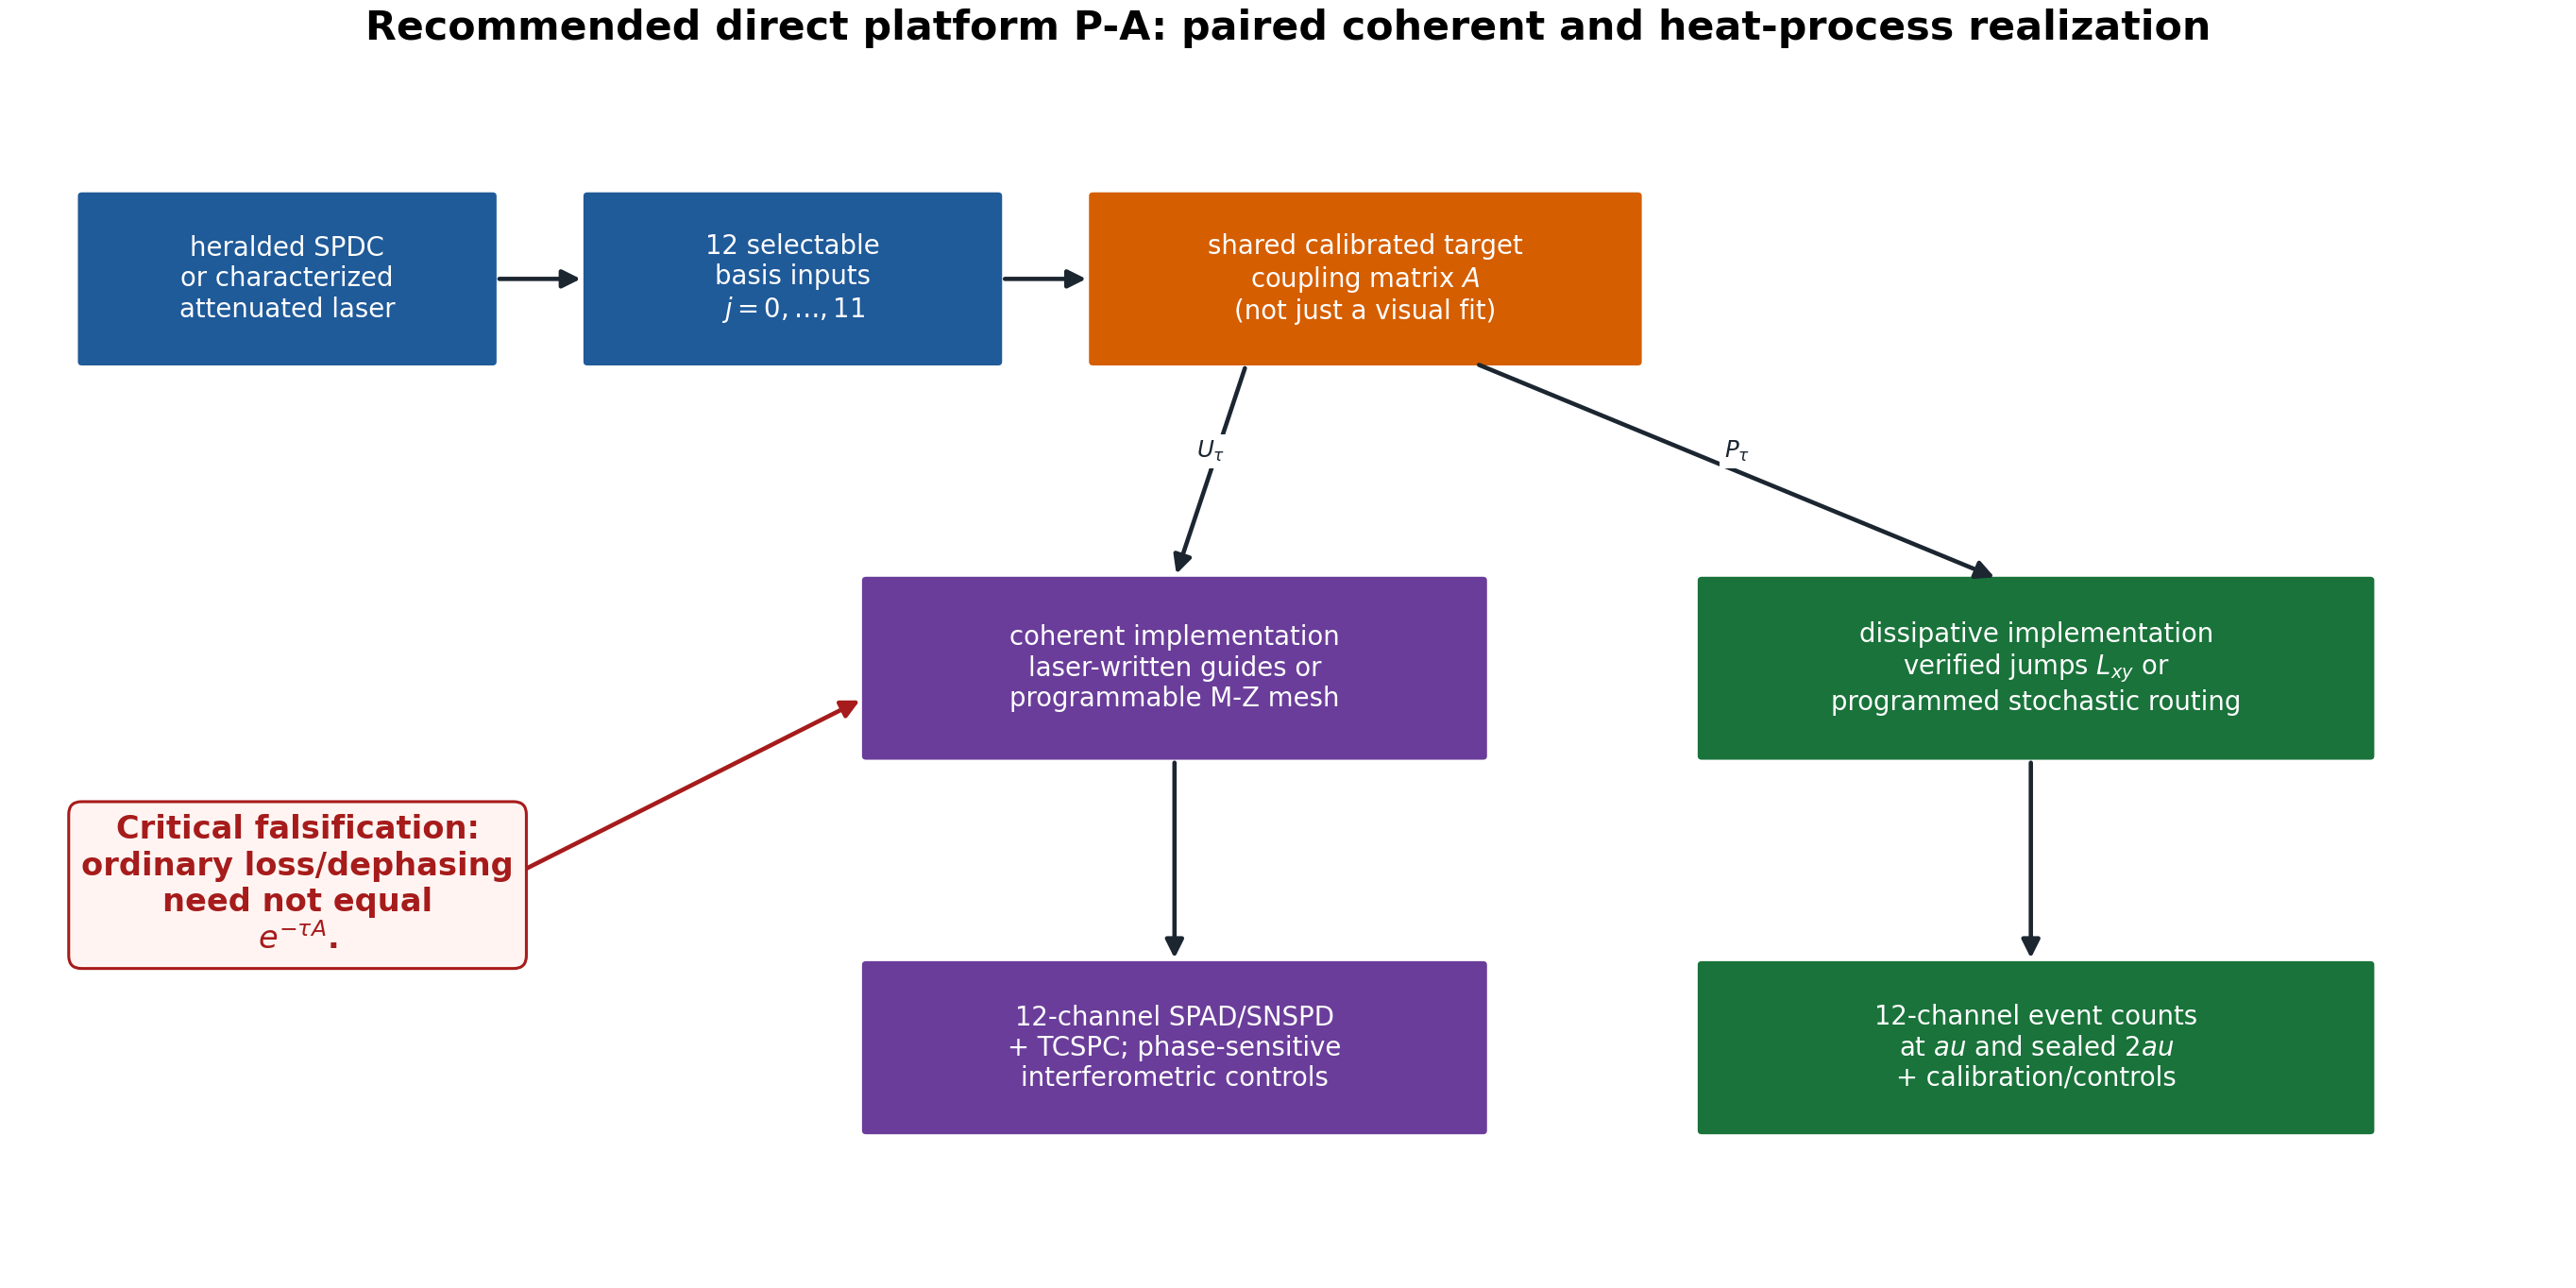
\includegraphics[width=0.96\textwidth]{FIN_Lab_P240_242_Transfer_Figures/platform_A_apparatus.png}
\caption{Recommended direct P-A architecture. Coherent propagation and heat flow require separately verified physical realizations of the common target generator.}
\end{figure}

\chapter{Platform P-B --- qubit Mach--Zehnder/\allowbreak{}Ramsey dephasing}

\section{Feasibility status}

\textbf{Feasibility hypothesis and auxiliary protocol.} A single qubit or two-path interferometer is suitable for the single/\allowbreak{}plus/\allowbreak{}echo identifiability problem and for testing detector blur, dephasing and temporal memory. It is not informationally complete for the twelve-node FIN generator.

\section{Apparatus}

\begin{itemize}
\item 
Mach--Zehnder interferometer, Ramsey-controlled qubit or equivalent two-level platform;

\item 
coherent source or qubit initialization;

\item 
AWG and microwave/\allowbreak{}optical pulse generation;

\item 
EOM, piezo phase control or qubit \(Z\) control;

\item 
single, plus and echo preparation/\allowbreak{}intervention sequences;

\item 
calibrated readout and detector-confusion matrix;

\item 
synchronized clock and event-level record;

\item 
optional environment/\allowbreak{}noise monitor.

\end{itemize}

\section{\texorpdfstring{Role of the quoted \(\tau_*=0.002\,\mathrm{s}\)}{Role of the quoted \_*=0.002\textbackslash{},s}}

The value \(0.002\,\mathrm{s}\) appeared in a conditional synthetic operational example. It is not a FIN-derived universal time and must not be imposed on a laboratory. The apparatus must select times from its independently calibrated coherence and control range.

\section{What P-B can test}

\begin{itemize}
\item 
whether single, plus and echo records identify declared dephasing and memory parameters;

\item 
whether an intermediate intervention changes a multitime record;

\item 
whether the apparatus blur model is stable on held-out runs;

\item 
whether environment models with identical one-time channels differ at two times.

\end{itemize}

\section{What P-B cannot establish}

It cannot reconstruct twelve transition columns, the \(C_{12}\) projective fingerprint, or the P242 semigroup holdout without a new, explicit encoding of twelve preparations and twelve outcomes.

\chapter{Platform P-C --- event-level double slit}

\section{Feasibility status}

\textbf{Feasibility hypothesis for an independent event record.} Time-resolved single-photon double-slit measurements with SPAD arrays have been demonstrated in the literature. P-C is therefore a strong candidate for testing the custody, raw-event and interference-analysis procedures. It is not by itself a realization of the finite FIN \(C_{12}\) operator.

\section{Apparatus}

\begin{itemize}
\item 
heralded SPDC single-photon source or characterized attenuated source;

\item 
spatial filtering and collimation;

\item 
two-slit mask with independently actuated left/\allowbreak{}right shutters;

\item 
four randomized configurations: both\_open, left\_only, right\_only, both\_closed;

\item 
fixed propagation geometry and alignment/\allowbreak{}stability monitors;

\item 
position-resolving EMCCD/\allowbreak{}ICCD or, preferably for direct timestamps, a SPAD array with TCSPC;

\item 
source trigger/\allowbreak{}herald detector where applicable;

\item 
independent dark-count, efficiency and point-spread calibration;

\item 
raw event storage.

\end{itemize}

Each event row must contain at least:

event\_id, timestamp\_utc, run\_id, subset, configuration, x\_detector, y\_detector, intervention

The raw record must be retained. A final image of interference fringes is insufficient.

\section{Four-configuration analysis}

Let \(N_{BO}(x)\), \(N_L(x)\), \(N_R(x)\) and \(N_{BC}(x)\) be efficiency- and exposure-corrected counts. An interference contrast can be formed from

\[
C(x)=N_{BO}(x)-N_L(x)-N_R(x)+N_{BC}(x).
\]

The contrast tests coherent cross terms relative to the registered controls. It does not identify \(A\) unless a twelve-mode mapping and propagation model were independently frozen.

\section{Mapping to the five duties}

\begin{center}
\begingroup\small
\setlength{\tabcolsep}{3.5pt}
\renewcommand{\arraystretch}{1.16}
\begin{longtable}{@{}p{0.420\textwidth}p{0.420\textwidth}@{}}
\toprule
\textbf{Duty} & \textbf{P-C implementation} \\
\midrule
\endhead
1 & four slit configurations, not the twelve P227 basis preparations \\
2 & timestamps and exposure/\allowbreak{}trigger calibration \\
3 & spatially resolved detector, not automatically the twelve-outcome vertex POVM \\
4 & event-by-event coordinate and time record \\
5 & a real independent bundle can satisfy P241 when signed and custody-separated \\
\bottomrule
\end{longtable}
\endgroup
\end{center}

\section{Physical boundary}

P-C can validate interference, background subtraction, raw-event storage and blind custody. A vanilla P-C bundle must make P242 return NOT\_SEMIGROUP\_READY. This is a safety feature.

\begin{figure}[htbp]
\centering
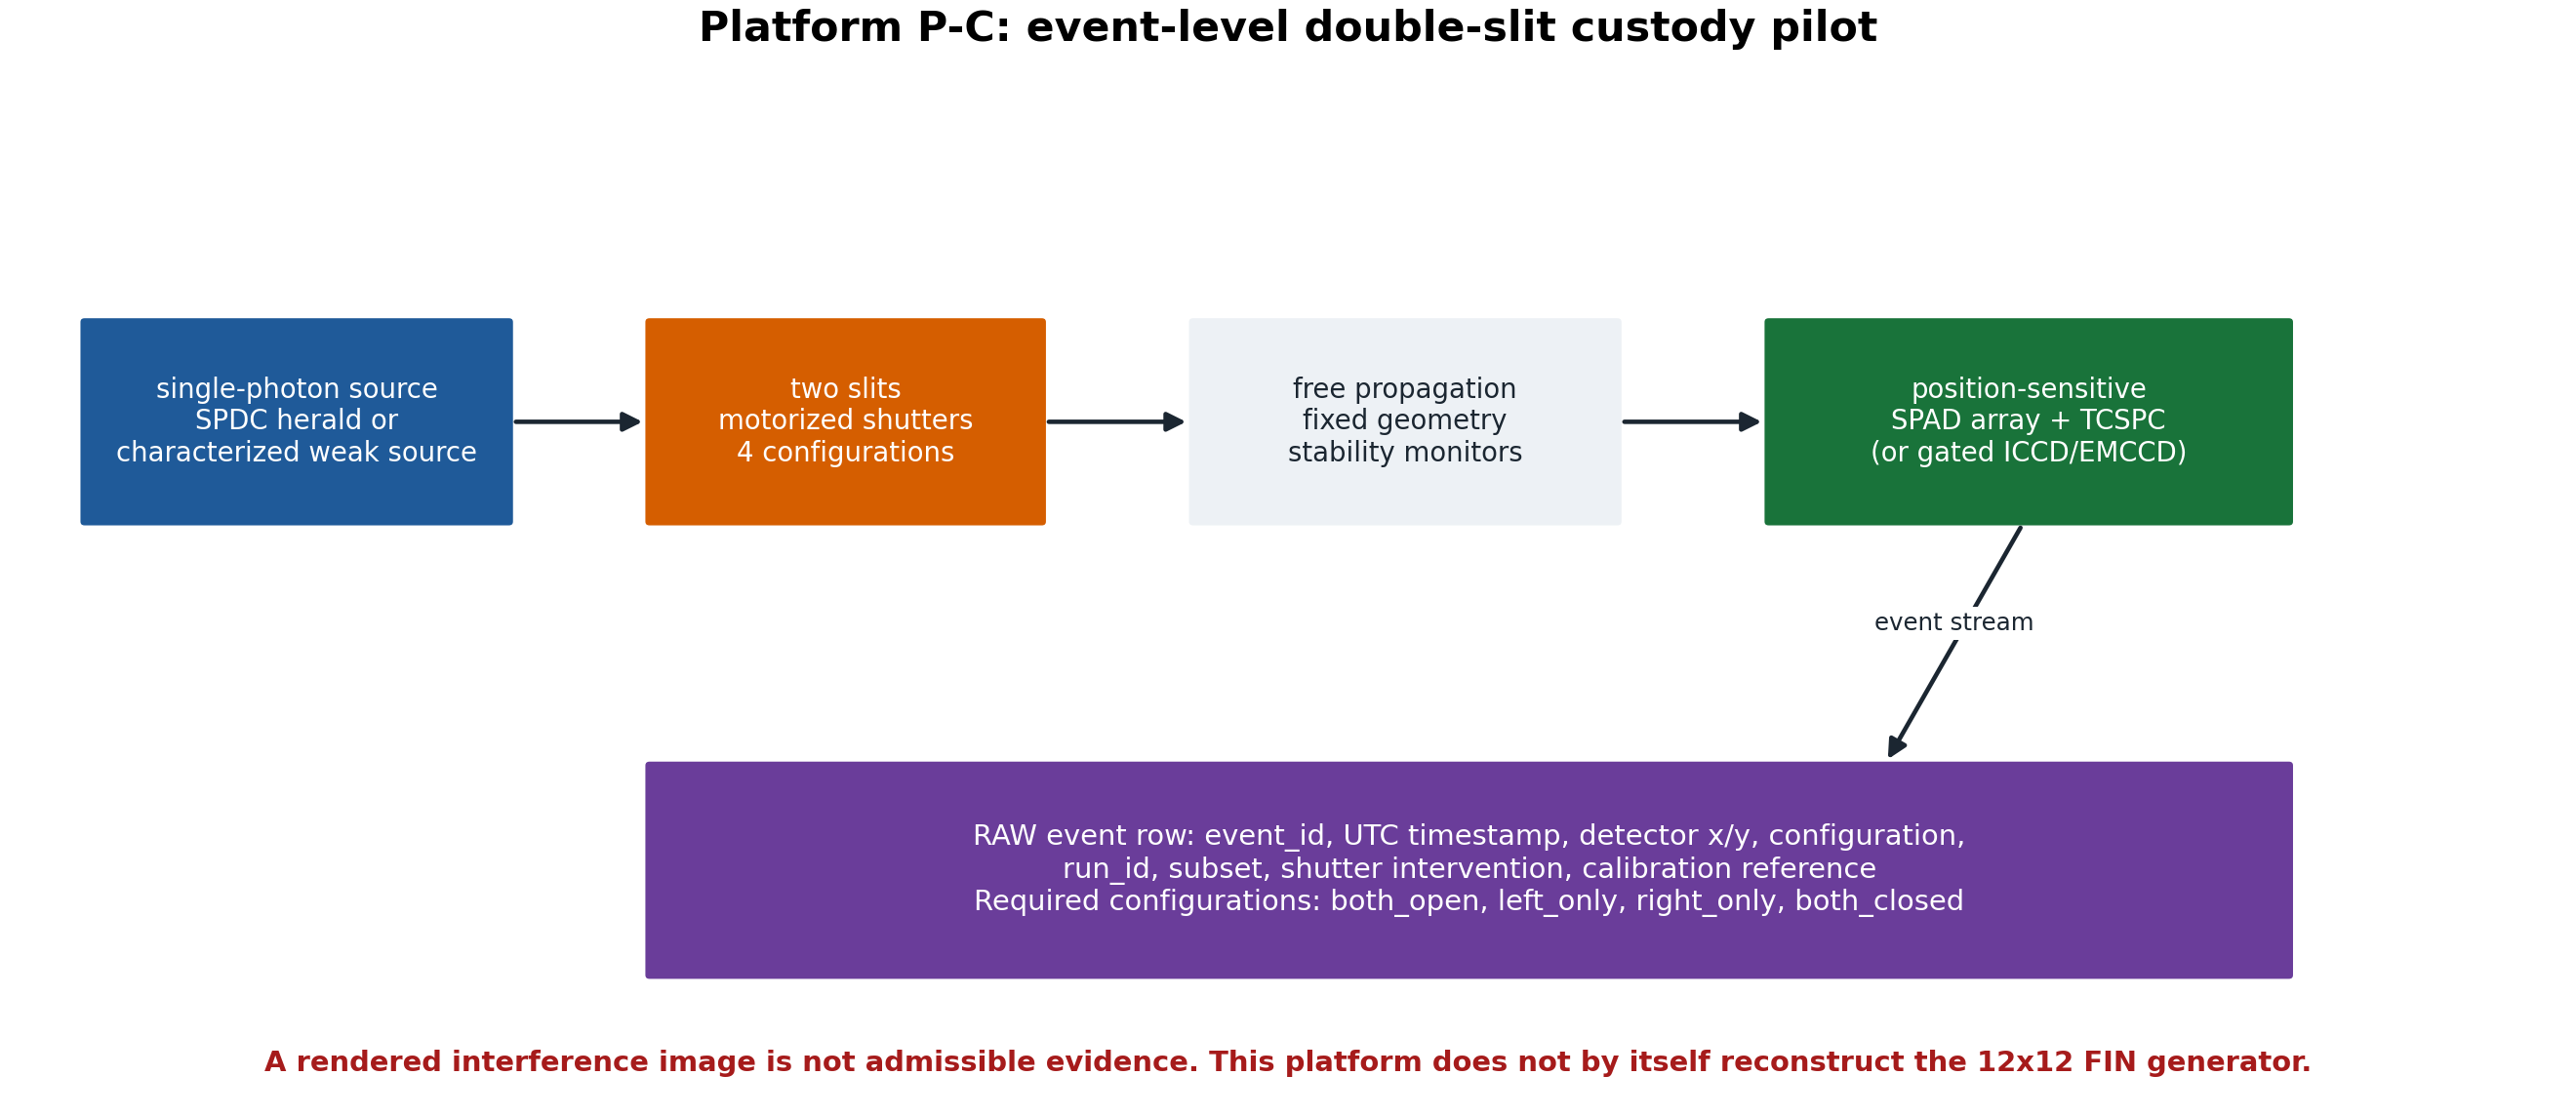
\includegraphics[width=0.96\textwidth]{FIN_Lab_P240_242_Transfer_Figures/platform_C_double_slit.png}
\caption{P-C event-level double-slit apparatus. Raw detections, four shutter configurations and calibrations are retained; a rendered image is not an admissible substitute.}
\end{figure}

\chapter{Blind-custody protocol}

The roles are disjoint:

\[
\mathrm{provider}\neq\mathrm{registrar}\neq\mathrm{analyst}.
\]

\section{Provider}

\begin{enumerate}
\item 
acquires raw events;

\item 
records all calibration, control and environment files;

\item 
does not see the frozen analysis result;

\item 
transfers the unmodified bundle to the registrar.

\end{enumerate}

\section{Registrar}

\begin{enumerate}
\item 
verifies event and metadata completeness;

\item 
computes SHA-256 for every file;

\item 
freezes the bundle digest;

\item 
verifies that preregistration predates acquisition;

\item 
seals the holdout;

\item 
signs bundle\_manifest.json with a detached GPG signature;

\item 
releases only the authorized split at each stage.

\end{enumerate}

\section{Analyst}

\begin{enumerate}
\item 
freezes P240/\allowbreak{}P242 code and the analysis-lock hash before unblinding;

\item 
does not possess the registrar signing key;

\item 
receives the calibration subset first;

\item 
performs no threshold or model repair after seeing the holdout;

\item 
runs P242 once.

\end{enumerate}

\section{One-run rule}

P242 creates an atomic ledger entry keyed by the bundle digest before reading the unblinded holdout. If an entry already exists, the pipeline refuses a second run. A failed run remains part of the scientific record.

\begin{figure}[htbp]
\centering
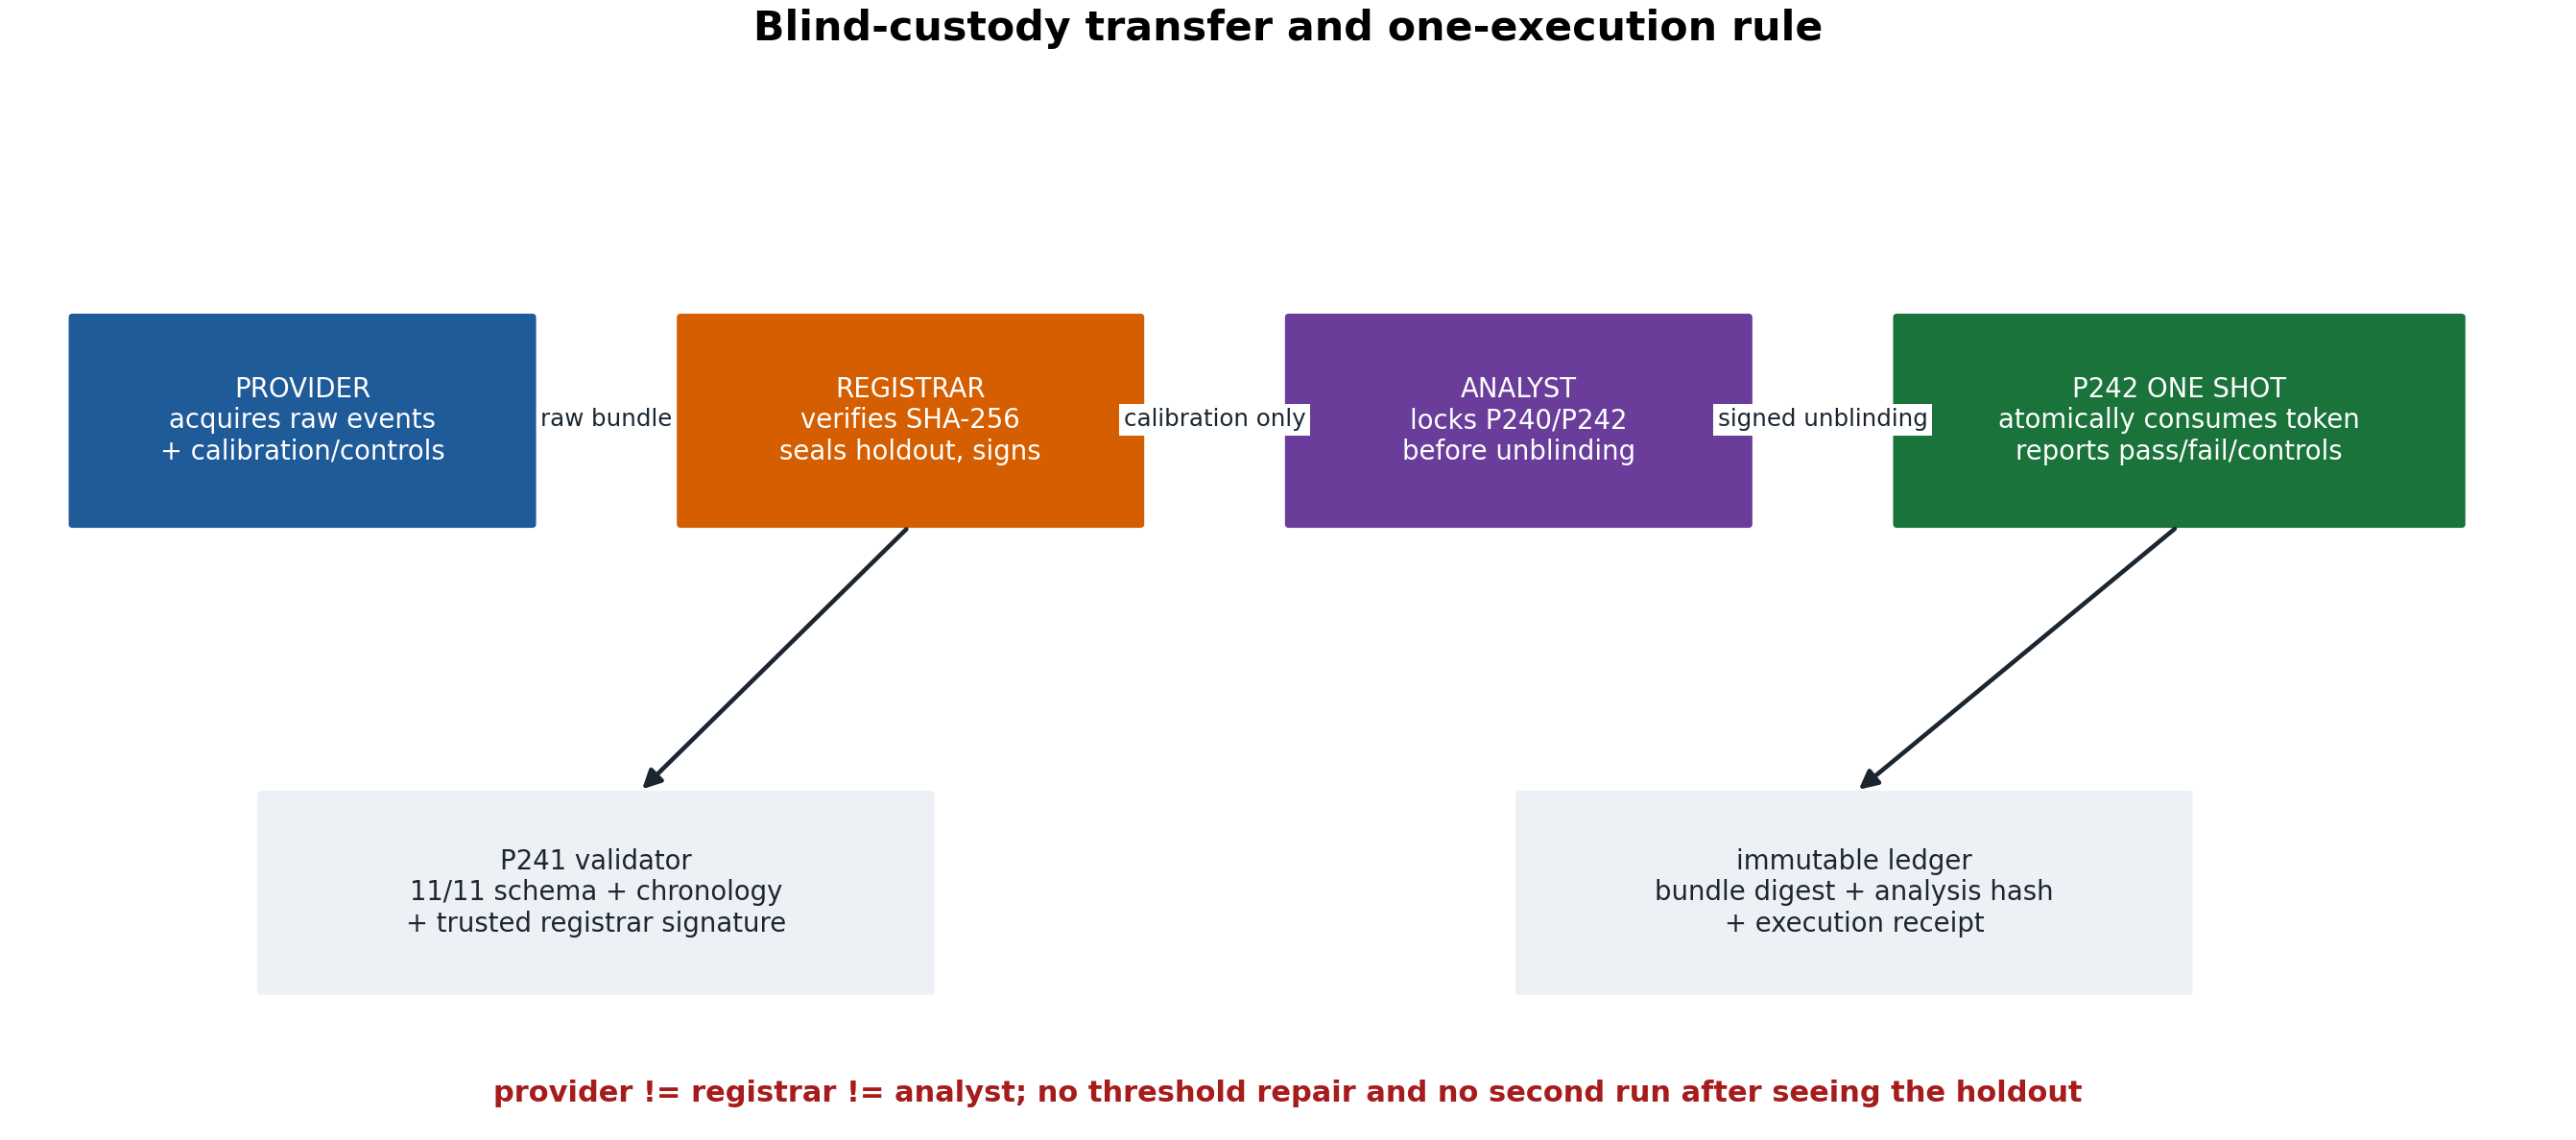
\includegraphics[width=0.96\textwidth]{FIN_Lab_P240_242_Transfer_Figures/custody_pipeline.png}
\caption{Provider, registrar and analyst remain distinct. The sealed holdout is released only after hashes and analysis code are frozen.}
\end{figure}

\par\medskip\hrule\medskip

\chapter{Recommended direct experiment}

\section{Experimental object}

The cleanest direct target is a paired twelve-state realization:

\[
\mathcal E_{\rm lab}
=
(\mathcal P_{12},C_\tau,\Phi_\tau,\mathcal M_{12},
\mathcal R,\mathcal C_{\rm custody}),
\]

where \(\mathcal P_{12}\) are twelve basis preparations, \(C_\tau\) is the calibrated clock, \(\Phi_\tau\) is the realized process, \(\mathcal M_{12}\) is the resolving measurement, \(\mathcal R\) is the event record and \(\mathcal C_{\rm custody}\) is the independent chain.

\section{Registered times}

Program 240 fixes

\[
\tau\lambda_{\max}=1,
\qquad
\tau=0.426952295949885
\]

in dimensionless units. The physical duration is determined by the measured rate scale:

\[
\tau_{\rm phys}=\frac{0.426952295949885}{\kappa}
\]

for the heat implementation.

The registered process times are:

\begin{center}
\begingroup\small
\setlength{\tabcolsep}{3.5pt}
\renewcommand{\arraystretch}{1.16}
\begin{longtable}{@{}p{0.232\textwidth}p{0.240\textwidth}p{0.388\textwidth}@{}}
\toprule
\textbf{Split} & \textbf{Dimensionless time} & \textbf{Purpose} \\
\midrule
\endhead
calibration & \(\tau\) & estimate \(\widehat P_\tau\) \\
sealed holdout & \(2\tau\) & test \(\widehat P_\tau^2\) \\
optional coherent diagnostic & \(\tau/4,\tau/2,\tau\) & linear-vs-quadratic escape and interference \\
\bottomrule
\end{longtable}
\endgroup
\end{center}

\section{Shot plan}

The recommended confirmatory allocation is:

\[
50\,000
\quad\text{events per preparation per registered heat time}.
\]

For twelve preparations and two times this is

\[
2\times12\times50\,000=1\,200\,000
\]

registered heat-process events, before controls and calibration.

A pilot may use \(10\,000\) events per preparation. It must not replace the confirmatory run after seeing pilot outcomes unless the adaptation was preregistered.

\section{Randomization}

\begin{itemize}
\item 
randomize preparation order in blocks;

\item 
interleave \(\tau\) calibration runs and control runs;

\item 
keep \(2\tau\) labels sealed from the analyst;

\item 
randomize double-slit shutter configurations if P-C is used;

\item 
record every dropped event and dead-time exclusion;

\item 
never reorder the archived raw stream.

\end{itemize}

\section{Calibration}

The following calibrations are mandatory:

\begin{enumerate}
\item 
physical clock and trigger latency;

\item 
twelve input preparation confusion matrix;

\item 
twelve output detector confusion/\allowbreak{}crosstalk matrix;

\item 
efficiency per channel;

\item 
dark-count and afterpulse rates;

\item 
dead time;

\item 
timing jitter;

\item 
coupling/\allowbreak{}process stability over the run;

\item 
spatial or mode relabelling map;

\item 
environmental monitors and background runs.

\end{enumerate}

Calibration parameters may be propagated as nuisance parameters. They may not be fitted separately to the sealed \(2\tau\) target.

\par\medskip\hrule\medskip

\chapter{Program 240 --- optimal spectral tomography}

\section{Exact time optimum}

Normalize the fastest nonzero generator rate to one and write

\[
x=\tau\lambda_{\max}.
\]

For a transition eigenvalue \(\mu=e^{-x}\), inverse-log recovery has local absolute-noise amplification

\[
g(x)=\frac{e^x}{x}.
\]

Since

\[
g'(x)=\frac{e^x(x-1)}{x^2},
\]

\(x=1\) is the unique positive minimizer. This proves the registered \(\tau\lambda_{\max}=1\) rule in the declared local absolute-noise model.

\section{Equal preparation allocation}

The target and declared risk are invariant under cyclic permutation of the twelve labels. For any allocation, average its twelve cyclic images. The average allocation is uniform. Convexity of the design risk implies that this symmetrization cannot increase risk. Thus a minimax allocation exists with equal shots for all twelve basis preparations.

This theorem does not say that uniform allocation remains optimal after detector asymmetry. Measured efficiency differences should be incorporated as preregistered costs or nuisance parameters.

\section{Nonasymptotic matrix concentration}

For each preparation \(j\), let \(X_{jr}\) be a one-hot outcome from \(P_\tau(\cdot|j)\) and let \(m\) shots be taken in every column. The raw transition error is a sum of independent rectangular matrices

\[
\widehat P-P
=
\sum_{j,r}
\frac{(X_{jr}-p_j)e_j^\mathsf T}{m}.
\]

Each summand has operator norm at most

\[
R\leq\frac{\sqrt2}{m}.
\]

The rectangular variance proxy satisfies

\[
v\leq\frac{n}{2m}.
\]

Matrix Bernstein therefore gives, with probability at least \(1-\alpha\),

\[
\|\widehat P-P\|_2
\leq
\sqrt{2v\log\frac{2n}{\alpha}}
+
\frac{2R}{3}\log\frac{2n}{\alpha}
=:\varepsilon.
\]

Symmetrization does not increase the operator error. If \(\varepsilon<\mu_{\min}(P)\), Weyl's theorem and the Lipschitz bound for the matrix logarithm give

\[
\|\widehat A-A\|_2
\lesssim
\frac{2\varepsilon}
{\tau(\mu_{\min}-\varepsilon)}.
\]

If this absolute rate error is \(\delta<\lambda_{\max}\), the normalized fingerprint error is bounded by

\[
\frac{2\delta}{\lambda_{\max}-\delta}.
\]

The bound is deliberately distribution free and conservative.

\section{Executed planning result}

At \(\tau\lambda_{\max}=1\):

\[
\lambda_{\min}(P_\tau)=e^{-1}=0.3678794411714421,
\]

and

\[
\lambda_{\min}(P_{2\tau})=e^{-2}=0.1353352832366125.
\]

Three hundred deterministic synthetic trials per shot level gave:

\begin{center}
\begingroup\small
\setlength{\tabcolsep}{3.5pt}
\renewcommand{\arraystretch}{1.16}
\begin{longtable}{@{}p{0.237\textwidth}p{0.228\textwidth}p{0.205\textwidth}p{0.189\textwidth}@{}}
\toprule
\textbf{Shots per preparation} & \textbf{Mean projective distance} & \textbf{95th percentile} & \textbf{Raw \(0.02\) pass rate} \\
\midrule
\endhead
10,000 & 0.016629 & 0.026915 & 0.7233 \\
25,000 & 0.009632 & 0.015303 & 0.9900 \\
50,000 & 0.006419 & 0.010079 & 1.0000 \\
\bottomrule
\end{longtable}
\endgroup
\end{center}

The distribution-free matrix-Bernstein/\allowbreak{}log sufficient count for a guaranteed \(0.02\) projective bound at \(\alpha=0.05\) is

\[
22\,565\,113
\]

shots per preparation. This is not the recommended practical count. It is an honest statement of the price of a broad worst-case guarantee. The \(50\,000\) plan is supported by target-model simulation and must be accompanied by the finite-count primary test and external controls.

\begin{figure}[htbp]
\centering
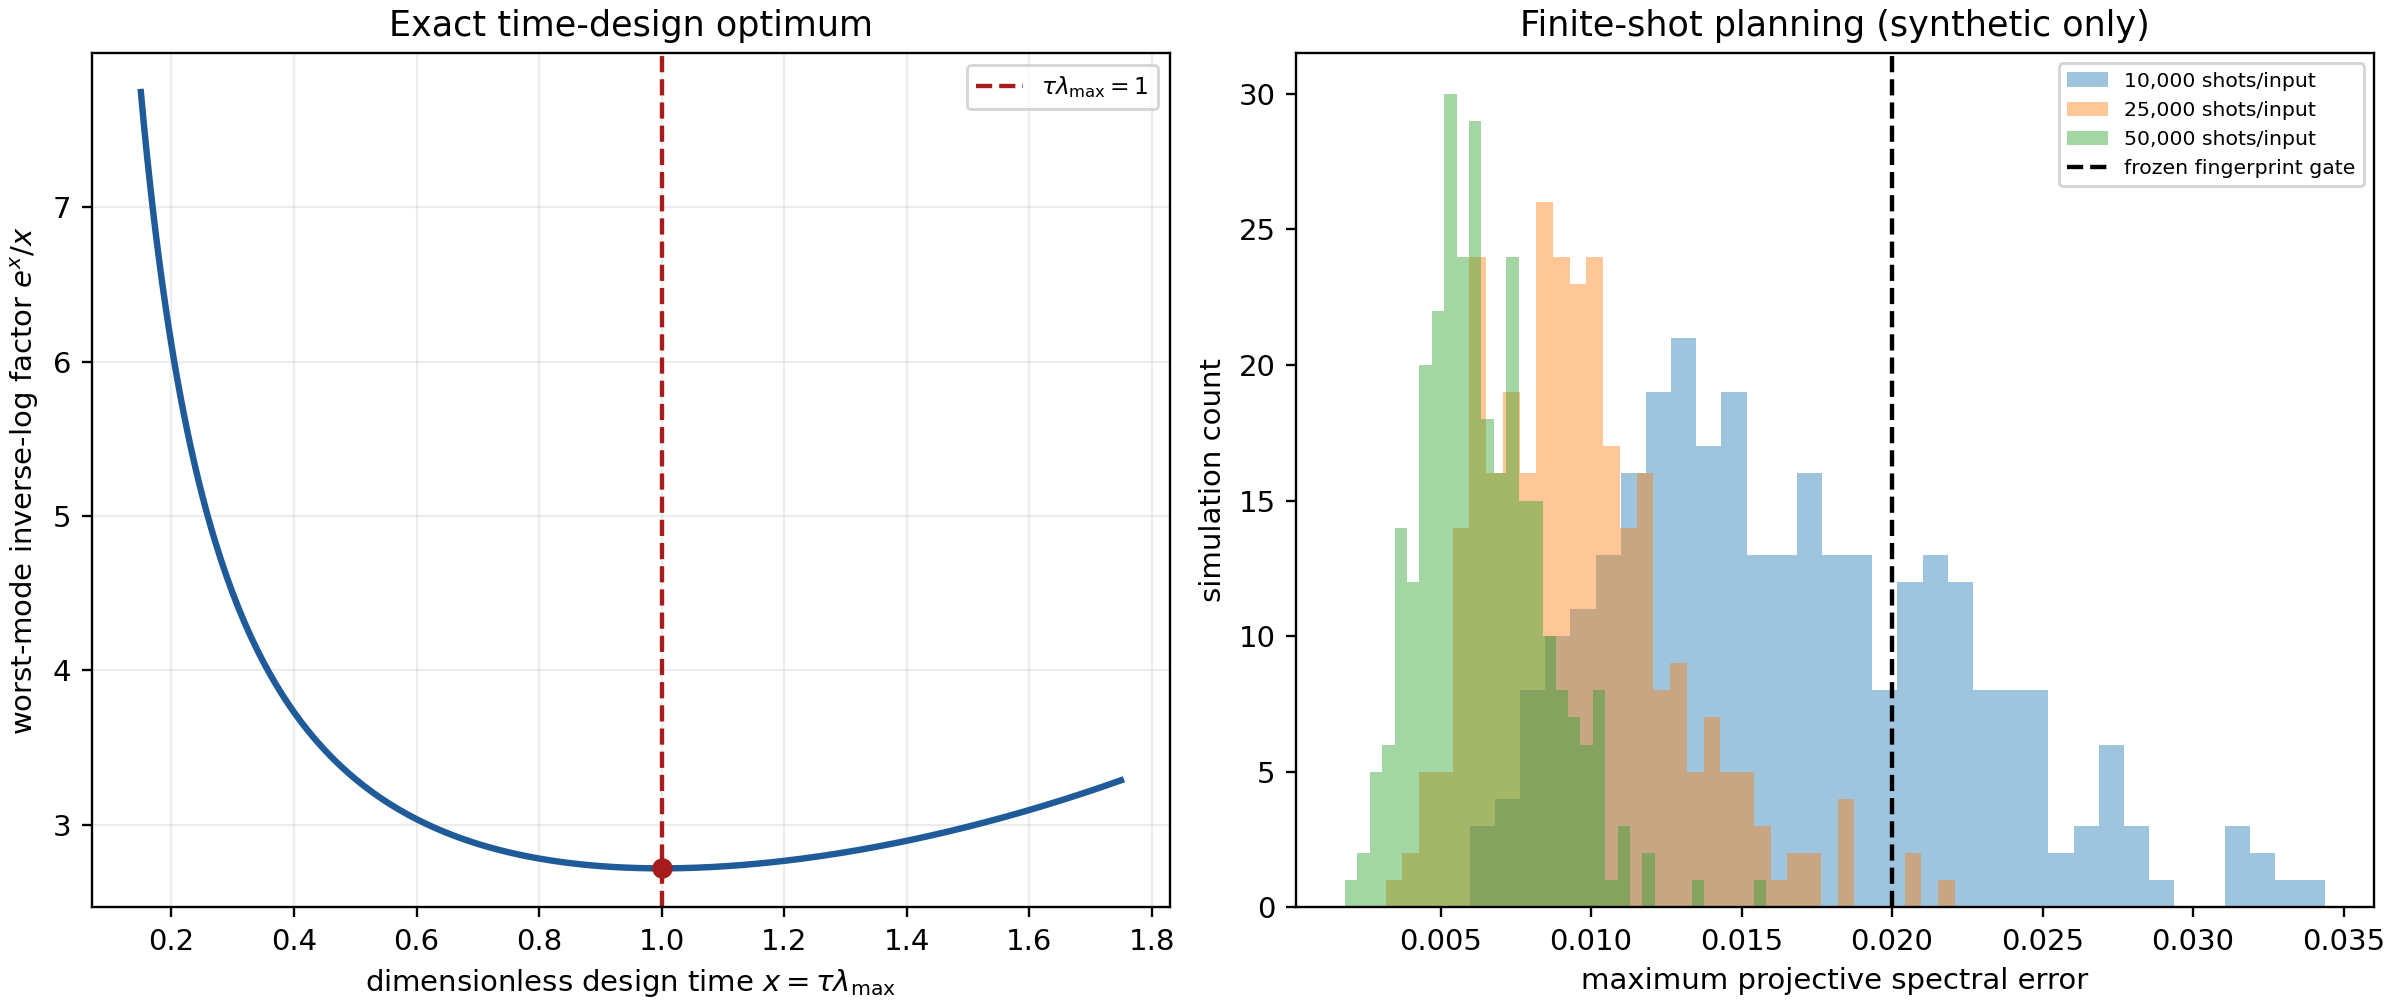
\includegraphics[width=0.96\textwidth]{FIN_Lab_P240_242_Transfer_Figures/p240_optimal_tomography.png}
\caption{Program 240: the exact fastest-mode time optimum and deterministic finite-shot planning distributions.}
\end{figure}

\par\medskip\hrule\medskip

\chapter{Program 241 --- executable validator}

\section{Eleven fields}

The validator checks:

\begin{enumerate}
\item 
independent provider identity and license;

\item 
immutable raw-event hashes;

\item 
ordered events or detection coordinates;

\item 
preparation or slit-configuration labels;

\item 
intervention or shutter labels;

\item 
clock and dimensional calibration;

\item 
detector geometry, efficiency, dark-count and blur calibration;

\item 
environment and background record;

\item 
negative controls;

\item 
held-out target committed before analysis;

\item 
provider--registrar--analyst role separation plus trusted registrar signature.

\end{enumerate}

\section{Bundle layout}

BUNDLE/\allowbreak{} bundle\_manifest.json bundle\_manifest.json.asc events.csv calibration.json controls.json environment.json preregistration.json

bundle\_manifest.json contains the SHA-256 of every declared file. Paths may not escape the bundle and symlinks are forbidden.

\section{Process event schema}

event\_id timestamp\_utc run\_id subset preparation\_id outcome\_id evolution\_multiple intervention

The production semigroup bundle must contain all preparations and outcomes \(0,\ldots,11\), evolution multiples \(1\) and \(2\), and the subsets calibration and holdout.

\section{Double-slit event schema}

event\_id timestamp\_utc run\_id subset configuration x\_detector y\_detector intervention

The required configurations are both\_open, left\_only, right\_only and both\_closed.

\section{Cryptographic boundary}

P241 requires a detached GPG signature of bundle\_manifest.json verified against a separately supplied trusted registrar keyring. This establishes file-level provenance relative to that key. It does not establish that the named people are genuinely independent. The collaboration must audit that fact institutionally.

\section{Commands}

Create empty templates:

python3 fin\_lab\_p241\_validator.py \\
--emit-template FIN\_Lab\_P241\_Transfer\_Template\_NEW

Validate a production bundle:

python3 fin\_lab\_p241\_validator.py BUNDLE \\
--signature BUNDLE/\allowbreak{}bundle\_manifest.json.asc \\
--trusted-keyring registrar-trustedkeys.gpg \\
--output admission\_certificate.json

Without all eleven fields and the trusted signature, the exit status is nonzero and P242 remains locked.

\par\medskip\hrule\medskip

\chapter{Program 242 --- one-shot analysis pipeline}

\section{Fail-closed prerequisites}

P242 requires:

\begin{itemize}
\item 
exact canonical analysis-lock file;

\item 
P241 signed 11/\allowbreak{}11 admission;

\item 
resource type heat\_process;

\item 
complete twelve-state \(\tau\) calibration record;

\item 
complete twelve-state sealed \(2\tau\) holdout;

\item 
preregistration committing the exact SHA-256 of the P242 analysis lock;

\item 
a registrar-controlled one-run ledger.

\end{itemize}

A standard double-slit bundle fails the semigroup-readiness check by design.

\section{Finite-count primary threshold}

For an \(n\)-category empirical distribution with \(m\) samples, the Bretagnolle--Huber--Carol bound is used in the form

\[
\|\widehat p-p\|_1
\leq
\sqrt{
\frac{2\left(n\ln2+\ln(1/\alpha)\right)}{m}
}
\]

with the failure budget unioned across twelve columns and the two registered times. For column-stochastic matrices,

\[
\|\widehat P_\tau^2-P_\tau^2\|_1
\leq
2\|\widehat P_\tau-P_\tau\|_1.
\]

At \(50\,000\) shots per preparation at both times, the registered maximum column-TV radius is

\[
0.0361142590.
\]

The labels are:

\begin{itemize}
\item 
FALSIFIED\_AT\_REGISTERED\_LEVEL if the observed statistic exceeds the registered bound;

\item 
NOT\_FALSIFIED\_AT\_REGISTERED\_LEVEL otherwise.

\end{itemize}

The second label is intentionally not VALIDATED.

\section{Negative controls}

P242 reports:

\begin{enumerate}
\item 
cyclic preparation-label shift;

\item 
reversed/\allowbreak{}misassigned time;

\item 
a nearest-neighbour \(C_{12}\) heat model whose single scale is fitted only on calibration data and then evaluated on the holdout.

\end{enumerate}

The collaboration should additionally report apparatus-specific controls, missing events and all exclusion counts.

\section{Atomic execution}

Before unblinded analysis, P242 creates

FIN\_P242\_EXECUTED\_<bundle\_digest>.lock

with an exclusive filesystem operation. A second attempt with the same bundle digest is refused.

\section{Production command}

python3 fin\_lab\_p242\_pipeline.py \\
--bundle BUNDLE \\
--signature BUNDLE/\allowbreak{}bundle\_manifest.json.asc \\
--trusted-keyring registrar-trustedkeys.gpg \\
--ledger-dir REGISTRAR\_LEDGER \\
--output FIN\_P242\_external\_result.json

No such command is executed in this release because no external signed bundle is supplied.

\par\medskip\hrule\medskip

\chapter{Statistical interpretation}

\section{Registered hypotheses}

The primary null is conditional:

\[
H_{\rm SG}:
\quad
P_{2\tau}=P_\tau^2
\quad
\text{for the realized, calibrated, time-homogeneous process}.
\]

The FIN fingerprint hypothesis is:

\[
H_{\rm FIN}:
\quad
\operatorname{spec}_+(A)/\lambda_{\max}
\quad
\text{matches the frozen strict target}.
\]

These are different hypotheses. A generic time-homogeneous Markov process may satisfy \(H_{\rm SG}\) and fail \(H_{\rm FIN}\).

\section{Decision table}

\begin{center}
\begingroup\small
\setlength{\tabcolsep}{3.5pt}
\renewcommand{\arraystretch}{1.16}
\begin{longtable}{@{}p{0.216\textwidth}p{0.225\textwidth}p{0.418\textwidth}@{}}
\toprule
\textbf{Semigroup} & \textbf{Fingerprint} & \textbf{Interpretation} \\
\midrule
\endhead
fail & any & registered time-homogeneous heat realization is falsified or apparatus nonstationarity/\allowbreak{}calibration failure occurred \\
not falsified & fail & a semigroup-like process exists but not the frozen strict fingerprint \\
not falsified & pass & registered implementation survives; compare alternatives and engineering provenance \\
pass only after refit & invalid & post-hoc repair; report original failure \\
\bottomrule
\end{longtable}
\endgroup
\end{center}

\section{Emulator boundary}

If the apparatus was programmed from the FIN matrix, a successful run shows that the matrix, control stack and analysis can be implemented. It is not an independent discovery of the matrix in nature. A stronger physical claim requires a domain selected independently of the FIN fit and competitive held-out performance against alternative models.

\section{Alternative models}

At minimum compare:

\begin{itemize}
\item 
nearest-neighbour \(C_{12}\) heat flow;

\item 
generic symmetric circulant generator with preregistered parameter count;

\item 
generic reversible Markov model;

\item 
coherent continuous-time quantum walk;

\item 
dephasing/\allowbreak{}open-system alternatives;

\item 
detector-confusion and clock-drift nuisance models.

\end{itemize}

Model flexibility must be penalized and all nuisance fitting must use calibration data only.

\par\medskip\hrule\medskip

\chapter{Double-slit relation to FIN duality}

The finite FIN two-path calculation on \(\mathbb Z_{12}\) uses a preparation

\[
\frac{|a\rangle|E_a\rangle+e^{i\phi}|b\rangle|E_b\rangle}{\sqrt2}
\]

and environment overlap

\[
\eta=\langle E_b|E_a\rangle.
\]

After \(U_t\), a vertex detector gives

\[
p_{\phi,\eta}(x,t)
=
\frac{|u_a|^2+|u_b|^2}{2}
+
\operatorname{Re}
\left(
\eta e^{-i\phi}u_a\overline{u_b}
\right).
\]

This formula demonstrates how preparation, environment record and detector enter an operational prediction. It is not a derivation of the continuum optical diffraction law.

The proposed physical double-slit setup P-C tests the same general operational distinction---coherent cross terms versus controlled one-slit and dark records---but not the FIN spectral fingerprint unless a separate, pre-frozen twelve-mode encoding is supplied.

The double-slit record is therefore valuable for:

\begin{itemize}
\item 
validating event-level acquisition;

\item 
measuring how interference builds from individual detections;

\item 
testing shutter and dark controls;

\item 
exercising provider/\allowbreak{}registrar/\allowbreak{}analyst custody;

\item 
demonstrating that a final image is not a sufficient scientific record.

\end{itemize}

It is not, by itself, the P242 semigroup experiment.

\par\medskip\hrule\medskip

\chapter{Apparatus acceptance tests}

Before evidence acquisition, the experimental team should demonstrate:

\section{Source}

\begin{itemize}
\item 
stable event rate;

\item 
measured single-photon or weak-source statistics;

\item 
herald timing where applicable;

\item 
no preparation-dependent source drift beyond preregistered tolerance.

\end{itemize}

\section{Preparation}

\begin{itemize}
\item 
each of twelve inputs addressable;

\item 
confusion matrix measured;

\item 
no omitted input;

\item 
randomized run order.

\end{itemize}

\section{Dynamics}

\begin{itemize}
\item 
coherent arm: independently reconstructed unitary or Hamiltonian within tolerance;

\item 
heat arm: independently reconstructed rate/\allowbreak{}process matrix;

\item 
stationarity across run blocks;

\item 
explicit evidence that dephasing/\allowbreak{}loss is not being confused with the target Markov channel.

\end{itemize}

\section{Measurement}

\begin{itemize}
\item 
twelve distinct outcomes;

\item 
detector efficiency, dark count, crosstalk and dead-time record;

\item 
position/\allowbreak{}vertex labels fixed before analysis;

\item 
raw timestamps retained.

\end{itemize}

\section{Clock}

\begin{itemize}
\item 
time base traceable to an external standard;

\item 
trigger offsets and jitter measured;

\item 
mapping from physical time to dimensionless \(\tau\) frozen.

\end{itemize}

\section{Custody}

\begin{itemize}
\item 
three distinct role identities;

\item 
registrar key established before data transfer;

\item 
every raw file hashed;

\item 
holdout sealed;

\item 
analysis-lock hash in preregistration;

\item 
one-execution ledger outside analyst control.

\end{itemize}

\par\medskip\hrule\medskip

\chapter{Falsification and stop rules}

The following outcomes must stop claim promotion:

\begin{enumerate}
\item 
any required P241 field fails;

\item 
registrar signature fails;

\item 
a file hash changes;

\item 
preparation or outcome coverage is incomplete;

\item 
the \(\tau\) and \(2\tau\) clocks are not commensurately calibrated;

\item 
process drift exceeds the preregistered stability tolerance;

\item 
the empirical transition spectrum is nonpositive where the logarithm is required;

\item 
\(T_{\rm CK}\) exceeds the registered finite-count radius;

\item 
the fingerprint fails \(0.02\);

\item 
a flexible alternative explains the holdout at least as well after complexity control;

\item 
the run requires a threshold, label or model change after unblinding.

\end{enumerate}

A failed implementation may motivate a new experiment. It does not permit a second P242 run on the same bundle.

\par\medskip\hrule\medskip

\chapter{What a successful experiment would and would not show}

\section{It would show}

\begin{itemize}
\item 
a real apparatus can realize the declared twelve-state process;

\item 
the event-level data satisfy the registered semigroup consistency test;

\item 
the projective spectrum agrees or disagrees with the strict finite target;

\item 
coherent and diffusive operational protocols can be compared under explicit preparations, clocks and instruments;

\item 
the transfer/\allowbreak{}custody procedure is reproducible by independent teams.

\end{itemize}

\section{It would not show}

\begin{itemize}
\item 
that the strict kernel is uniquely selected by fundamental physics;

\item 
that the legacy kernel is physically transferred to the strict kernel;

\item 
that the dimensional constants emerge from FIN;

\item 
that an absolute orientation or selector emerges;

\item 
that a continuum, Lorentz symmetry, gauge sector, Standard Model or gravity has been derived;

\item 
that FIN is a Theory of Everything.

\end{itemize}

The strongest permissible positive conclusion after an emulator success is:

\begin{quote}\itshape
The frozen finite FIN operator and its registered operational heat/\allowbreak{}coherent tests were implemented and survived the declared held-out analysis on this apparatus.

\end{quote}

\par\medskip\hrule\medskip

\chapter{Handoff responsibilities}

\section{Theoretical physicist}

\begin{itemize}
\item 
verify the matrix convention and spectral target;

\item 
inspect the coherent and Lindblad/\allowbreak{}stochastic realizations;

\item 
define admissible nuisance models;

\item 
check that the physical channel corresponds to the declared mathematical object.

\end{itemize}

\section{Experimental physicist}

\begin{itemize}
\item 
select hardware and characterize limitations;

\item 
establish physical time and detector calibration;

\item 
validate state preparation and measurement;

\item 
preserve raw events and stability monitors.

\end{itemize}

\section{Statistician /\allowbreak{} analyst}

\begin{itemize}
\item 
freeze the analysis hash;

\item 
inspect P240 bounds and practical power;

\item 
preserve the registered failure budget;

\item 
report alternatives and non-rejections correctly.

\end{itemize}

\section{Independent registrar}

\begin{itemize}
\item 
maintain the trusted signing key and ledger;

\item 
verify chronology and hashes;

\item 
seal/\allowbreak{}unseal the holdout;

\item 
prevent repeated analysis of the same bundle.

\end{itemize}

\section{Repository maintainer}

\begin{itemize}
\item 
preserve source, tests, locks, manifest and PDF hashes;

\item 
do not replace external events with generated examples;

\item 
do not change P242 after the preregistration hash is published.

\end{itemize}

\par\medskip\hrule\medskip

\chapter{Executable inventory}

\begin{center}
\begingroup\small
\setlength{\tabcolsep}{3.5pt}
\renewcommand{\arraystretch}{1.16}
\begin{longtable}{@{}p{0.420\textwidth}p{0.420\textwidth}@{}}
\toprule
\textbf{File} & \textbf{Function} \\
\midrule
\endhead
fin\_lab\_p240\_optimal\_tomography.py & target construction, time/\allowbreak{}allocation theorem, concentration bounds and synthetic planning \\
FIN\_Lab\_P240\_Design\_Lock.json & canonical registered design \\
FIN\_Lab\_P240\_Optimal\_Tomography\_Results.json & machine-readable executed P240 results \\
fin\_lab\_p241\_validator.py & eleven-field schema/\allowbreak{}hash/\allowbreak{}chronology/\allowbreak{}signature validator \\
FIN\_Lab\_P241\_Transfer\_Template/\allowbreak{} & empty transfer templates; not evidence \\
fin\_lab\_p242\_pipeline.py & fail-closed one-run external analysis \\
FIN\_Lab\_P242\_Analysis\_Lock.json & canonical frozen P242 analysis \\
test\_fin\_lab\_p240\_242.py & regression/\allowbreak{}falsification tests \\
fin\_lab\_transfer\_figures.py & code-native scientific diagrams \\
\bottomrule
\end{longtable}
\endgroup
\end{center}

The laboratory should archive the exact SHA-256 manifest delivered with this PDF.

\par\medskip\hrule\medskip

\chapter{Reproduction commands}

Run P240:

MPLCONFIGDIR=/\allowbreak{}tmp/\allowbreak{}matplotlib-finlab \\
python3 fin\_lab\_p240\_optimal\_tomography.py --replicates 300

Regenerate the analysis lock:

python3 fin\_lab\_p242\_pipeline.py --write-lock-only

Run the tests:

MPLCONFIGDIR=/\allowbreak{}tmp/\allowbreak{}matplotlib-finlab \\
python3 -m unittest -v test\_fin\_lab\_p240\_242.py

Expected result:

Ran 18 tests OK

The P242 production command must not be run until P241 has admitted a genuine external bundle.

\par\medskip\hrule\medskip

\chapter{Literature and methodological anchors}

The apparatus proposals use established frameworks. Their use here does not claim novelty for those frameworks.

\begin{enumerate}
\item 
E. Farhi and S. Gutmann, "Quantum computation and decision trees," \emph{Physical Review A} \textbf{58}, 915--928 (1998). https:/\allowbreak{}/\allowbreak{}doi.org/\allowbreak{}10.1103/\allowbreak{}PhysRevA.58.915

\item 
H. B. Perets et al., "Realization of quantum walks with negligible decoherence in waveguide lattices," \emph{Physical Review Letters} \textbf{100}, 170506 (2008). https:/\allowbreak{}/\allowbreak{}doi.org/\allowbreak{}10.1103/\allowbreak{}PhysRevLett.100.170506

\item 
W. R. Clements et al., "Optimal design for universal multiport interferometers," \emph{Optica} \textbf{3}, 1460--1465 (2016). https:/\allowbreak{}/\allowbreak{}doi.org/\allowbreak{}10.1364/\allowbreak{}OPTICA.3.001460

\item 
F. Caruso et al., "Fast escape of a quantum walker from an integrated photonic maze," \emph{Nature Communications} \textbf{7}, 11682 (2016). https:/\allowbreak{}/\allowbreak{}doi.org/\allowbreak{}10.1038/\allowbreak{}ncomms11682

\item 
P. Kolenderski et al., "Time-resolved double-slit interference pattern measurement with entangled photons," \emph{Scientific Reports} \textbf{4}, 4685 (2014). https:/\allowbreak{}/\allowbreak{}doi.org/\allowbreak{}10.1038/\allowbreak{}srep04685

\item 
F. A. Pollock et al., "Non-Markovian quantum processes: Complete framework and efficient characterization," \emph{Physical Review A} \textbf{97}, 012127 (2018). https:/\allowbreak{}/\allowbreak{}doi.org/\allowbreak{}10.1103/\allowbreak{}PhysRevA.97.012127

\item 
P. Taranto et al., "The structure of quantum stochastic processes with finite Markov order," \emph{Physical Review A} \textbf{99}, 042108 (2019). https:/\allowbreak{}/\allowbreak{}doi.org/\allowbreak{}10.1103/\allowbreak{}PhysRevA.99.042108

\item 
J. A. Tropp, "User-friendly tail bounds for sums of random matrices," \emph{Foundations of Computational Mathematics} \textbf{12}, 389--434 (2012). https:/\allowbreak{}/\allowbreak{}doi.org/\allowbreak{}10.1007/\allowbreak{}s10208-011-9099-z

\item 
T. Weissman et al., "Inequalities for the L1 deviation of the empirical distribution," Hewlett-Packard Laboratories Technical Report HPL-2003-97 (2003).

\item 
B. Bylander et al., "Noise spectroscopy through dynamical decoupling with a superconducting flux qubit," \emph{Nature Physics} \textbf{7}, 565--570 (2011). https:/\allowbreak{}/\allowbreak{}doi.org/\allowbreak{}10.1038/\allowbreak{}nphys1994

\end{enumerate}

\par\medskip\hrule\medskip

\chapter{Final transfer statement}

The finite mathematical result is strong and narrow:

\[
A=sI-W
\]

is a positive connected weighted-graph Laplacian for the frozen strict twelve-node FIN profile, and the same spectrum supports coherent and diffusive functional calculi.

The missing bridge is not another formula in \(A\). It is an independently implemented and calibrated operational process with a real record.

This release supplies the part that can honestly be supplied before a laboratory acts:

\[
\boxed{
\text{P240 design lock}
\;+\;
\text{P241 signed validator}
\;+\;
\text{P242 one-shot pipeline}
}
\]

The fifth duty remains deliberately empty. Only an independent experimental collaboration can fill it.


\clearpage
\chapter*{Release reproducibility}
\addcontentsline{toc}{chapter}{Release reproducibility}
\begin{Verbatim}[fontsize=\small]
MPLCONFIGDIR=/tmp/matplotlib-finlab \
python3 fin_lab_p240_optimal_tomography.py --replicates 300

python3 fin_lab_p242_pipeline.py --write-lock-only

MPLCONFIGDIR=/tmp/matplotlib-finlab \
python3 -m unittest -v test_fin_lab_p240_242.py
\end{Verbatim}

Expected test result: 18 tests, all passing.  No P242 production execution is
part of this release because no signed external P241 bundle is supplied.

\medskip
\noindent\textbf{Suggested citation:}

\.Zuchowski, K. (2026). \emph{FIN Laboratory Transfer Package: P240 Optimal
Tomography, P241 Blind-Custody Validator, and P242 One-Shot Pipeline}
(Release 10.21; Version 1.0.0) [Preprint and executable specification].
Independent Researcher --- Fractal Information Theory Project.
\end{document}
